\chapter{单变量函数}
前面中我们已经说明了如何由量的度量而产生实数
系。在这一章中我们要进一步说明如何用变数符号去表达变
量,用变数之间的函数关系去表达变量之间的关联。变数是
变量的抽象,函数是变量相互关系的抽象。在这一章里我们
还要运用极限来分析和确立连续函数的概念。

\section{函数的概念}
\subsection{变数和变域}
在研究自然现象时,人们会遇到许多不同的物理量,如
时间、长度、体积、速度、质量、力等等。按照给定条件,
能取许多不同数值的量叫做\textbf{变量};而只取一个数值的量叫做
\textbf{常量},用来表达变量的符号叫做\textbf{变数}。习惯上常用$x,y,
z$等字母表示变数,从纯数学的观点来说,一个变数就是一
个“能取许多不同数值”的符号,它所能取的所有数值构成
一个集合,叫做它的\textbf{变域}。如果变数$x$的变域已经给出,我
们就认为变数$x$是已知的。一般说来,任何数集可以当作变
数的变域。常会遇到取所有自然数的变数$n$, 譬如数列中的
项数。可是在现实生活中,我们通常研究的是连续变化的变
数,如动点所经过的路程及所花的时间等物理量,就是这种
变数的原形,数的区间就是这一类变数的变域,最常用的区
间是以两个实数$a$与$b$ $(a<b)$——它的两个端点——为界
限的有限区间,两个端点本身可以包含在区间内,也可以不
包含在内。因此我们可以把区间分为:
\begin{itemize}
    \item 开区间$(a,b)$就是$\{x|a<x<b\}$;
    \item  闭区间$[a,b]$就是$\{x|a\le x\le b\}$;
    \item  半开区间$(a,b]$就是$\{x|a<x\le b\}$;
    $[a,b)$就是$\{x|a\le x<b\}$。
\end{itemize}
在上述各种情形,数$b-a$为区间的长度。

常量可以看作变量的特殊情形,它的变域是由一个数组
成的集合$\{x|x=a\}$。

数轴上的线段是数的区间的几何表示,图示开区间如图
8.1或8.2。

在点$a,b$处的圆圈或圆括号表示从区间去掉这两个
数。在两个圆圈之间的粗线段表示在$a,b$之间的一切数$x$。
图示闭区间如图8.3。
图示半开区间如图8.4、8.5,每一种情形都只包含出现
有方括号的数,以及在$a,b$之间的一切实数。
\begin{figure}[htp]\centering
    \begin{minipage}[t]{0.48\textwidth}
    \centering
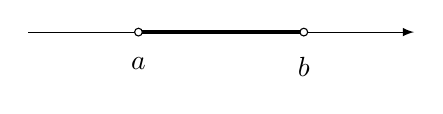
\begin{tikzpicture}[>=latex, scale=.7]
       \draw[->] (0.5,0)--(7.5,0);
       \draw[ultra thick] (2.5,0)node[below=5pt]{$a$}--(5.5,0)node[below=5pt]{$b$};
       \draw (2.5,0)[fill=white] circle (2pt);
        \draw (5.5,0)[fill=white] circle (2pt);
    \end{tikzpicture}
    \caption{}
    \end{minipage}
    \begin{minipage}[t]{0.48\textwidth}
    \centering
    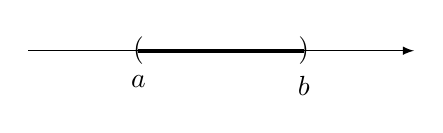
\begin{tikzpicture}[>=latex, scale=.7]
        \draw[->] (0.5,0)--(7.5,0);
        \draw[ultra thick] (2.5,0)node[below=5pt]{$a$}--(5.5,0)node[below=5pt]{$b$};
        \node at (2.5,0){$($}; \node at (5.5,0){$)$};
    \end{tikzpicture}
    \caption{}
    \end{minipage}
    \end{figure}

\begin{figure}[htp]\centering
    \begin{minipage}[t]{0.48\textwidth}
    \centering
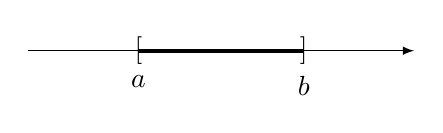
\begin{tikzpicture}[>=latex, scale=.7]
    \draw[->] (0.5,0)--(7.5,0);
    \draw[ultra thick] (2.5,0)node[below=5pt]{$a$}--(5.5,0)node[below=5pt]{$b$};
    \node at (2.5,0){$[$}; \node at (5.5,0){$]$};
    \end{tikzpicture}
    \caption{}
    \end{minipage}
    \begin{minipage}[t]{0.48\textwidth}
    \centering
    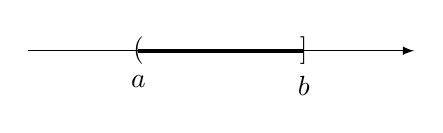
\begin{tikzpicture}[>=latex, scale=.7]
        \draw[->] (0.5,0)--(7.5,0);
        \draw[ultra thick] (2.5,0)node[below=5pt]{$a$}--(5.5,0)node[below=5pt]{$b$};
        \node at (2.5,0){$($}; \node at (5.5,0){$]$};
    \end{tikzpicture}
    \caption{}
    \end{minipage}
    \end{figure}

\begin{figure}[htp]\centering
    \begin{minipage}[t]{0.48\textwidth}
    \centering
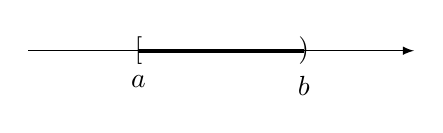
\begin{tikzpicture}[>=latex, scale=.7]
    \draw[->] (0.5,0)--(7.5,0);
    \draw[ultra thick] (2.5,0)node[below=5pt]{$a$}--(5.5,0)node[below=5pt]{$b$};
    \node at (2.5,0){$[$}; \node at (5.5,0){$)$};
    \end{tikzpicture}
    \caption{}
    \end{minipage}
    \begin{minipage}[t]{0.48\textwidth}
    \centering
    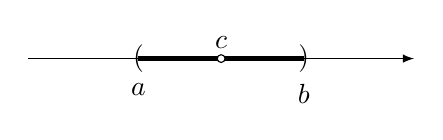
\begin{tikzpicture}[>=latex, scale=.7]
        \draw[->] (0.5,0)--(7.5,0);
        \draw[ultra thick] (2.5,0)node[below=5pt]{$a$}--(5.5,0)node[below=5pt]{$b$};
        \node at (2.5,0){$($}; \node at (5.5,0){$)$};
        \draw (4,0)[fill=white] circle (2pt)node[above]{$c$};
    \end{tikzpicture}
    \caption{}
    \end{minipage}
    \end{figure}

有时也要考虑无穷区间,用符号$-\infty,+\infty$作为一端或
两端,它们的记号和上面所引进的相类似,例如$(-\infty,+\infty)$
是全体实数集合$\{x|x\in\mathbb{R}\}$, 区间$(a,+\infty)$表示集
合$\{x|x>a\}$, 区间$(-\infty,b]$表示集合$\{x|x\le b\}$. 无穷区间
在几何上可用两端无限伸延的直线或一端无限伸延的射线来
表示。

以后我们要常用到一点的邻域的概念。\textbf{$c$点的邻域}是包
含$c$点的任何开区间$(a,b)$, 而$c$点的去心邻域指去掉$c$
点的任何$c$点的邻域。它的图象如图8.6。

$c$点的去心邻域可写成$(a,c)\cup (c,b)$. 我们常把
$c$点的邻域写成对称的形式:$(c-r,c+r)$, 对任何
$r>0$, 并且称它为\textbf{$c$点的对称邻域}。

\begin{example}
    试写出含于区间$(1,5)$中$\pi$的对称邻域。
$\left(\pi-\frac{1}{2},\pi+\frac{1}{2}\right)$是含于$(1,5)$的$\pi$对称邻域。此外
$(\pi-1,\pi+1)$, $\left(\pi-\frac{3}{2},\pi+\frac{3}{2}\right)$, $(\pi-0.01,\pi+0.01)$
等都是含于$(1,5)$中的对称邻域。
\end{example}

\subsection{函数的定义}
我们已经在第三册研究过许多函数,例如多项式函数、
三角函数,由于函数这个概念的重要性,并且它将是我们
的主要研究对象,因此需要回忆一般的函数的定义,下面我
们从数集之间的多对一(包括一对一)的关系重新给出函数
定义。

\begin{blk}{定义}
     设有数集$A,B$, 如果有一对应关系或法则$f$存
在,对于$A$的任何一个数$x$, 有数集$B$中唯一的一个数$y$与之
对应,我们就称给出了一个从数集$A$到数集$B$内的函数$f$, 用
\[f:A\mapsto B\]
表示,并写成$y=f(x),\; (x\in A)$, 此时称$f(x)$为函数$f$在$x$的
函数值,并称$A$为函数$f$的\textbf{定义域}。又当$x$取遍$A$中的数时,
函数值$f(x)$全体也构成一个数集,称为函数$f$的\textbf{值域},记作
\[f(A)=\{f(x)|x\in A\}\]
要注意的是在构造一个函数$f:A\mapsto B$的时候,$f(A)$不一定等
于$B$, 而是$B$的一个真子集,即$f(A)\subset B$。
\end{blk}



\begin{example}
设$\mathbb{R}$是实数集,函数$f:\mathbb{R}\mapsto\mathbb{R}$定义为
\[f(x)=\frac{2x}{x^2+1},\quad x\in(-\infty,+\infty)\]
求它的值域。
\end{example}

\begin{solution}
    方程$f(x)=\frac{2x}{x^2+1}$等价于
    \begin{equation}
        yx^2-2x+y=0
    \end{equation}
根据函数的值域定义,任给$y\in f(\mathbb{R})$, 方程(8.1)必有实数
解,而方程(8.1)有实数解的充要条件是
\[\Delta=1-y^2\ge 0\]
即:$-1\le y\le 1$,所以
\[f(\mathbb{R})=\{f(x)|-1\le f(x)\le 1\}\subset \mathbb{R}\]
\end{solution}

在函数的定义中包含三个要素,即\textbf{定义域},\textbf{多对一的对
应法则}和\textbf{函数值所在的数集}。应养成一个习惯,当给定一个
函数时,必须指明它的定义域。在实际问题中,函数的定义
域是根据实际意义来确定的,例如温度计刻有华氏温标度数
$F$和摄氏温标度数$c$,因为不存在低于绝对零度的温度,因
此,这两个度数之间的函数$\varphi$是
\[F=\varphi(c)=\frac{9}{5}c+32,\quad c\in (-273,+\infty)\]

以后,当我们只在数学上,一般地研究一个具体解析式
子规定的函数关系时,如果定义域$A$没有被指明,那么函数
的定义域是使解析式子具有数值意义的所有$x$的数值组成的
自然定义域,函数$y$的值域通常是不指出的,因为由对应的
规律本身就可以确定函数的值域。


\begin{example}
    求下列函数定义域:
\begin{multicols}{2}
\begin{enumerate}
    \item $f(x)=\frac{\sqrt{1-x}}{x}$
    \item $g(x)=\sqrt{x^2-1}$
\end{enumerate}
\end{multicols}
\end{example}

\begin{solution}
    \begin{enumerate}
        \item \[\text{函数$f$有意义}\Leftrightarrow \begin{cases}
    1-x \ge 0\\
    x\ne 0
\end{cases}\Rightarrow\quad x\le 1, \quad x\ne 0\]
$\therefore\quad $函数$f$的定义域为$(-\infty,0)\cup(0,1]$。

\item \[\text{函数$g$有意义}\Leftrightarrow x^2-1\ge 0 \Rightarrow\quad x\le 1, \text{ 或 } x\ge 1\]
$\therefore\quad $函数$g$的定义域为$(-\infty,-1]\cup[1,+\infty)$。
    \end{enumerate}
\end{solution}

\subsection{相等的函数}
怎样的两个函数是相等的函数?在数学中,有些函数可
以用不同的方式来定义,例如,函数$f:\mathbb{R}\mapsto \mathbb{R}^+\cup\{0\}$是由
$f(x)=|x|$规定的,而函数$g:\mathbb{R}\mapsto \mathbb{R}^+\cup\{0\}$是由$g(x)=\sqrt{x^2}$规定的,这里表示$f(x)$与$g(x)$的式子全不同,但是对
于它们的相同的定义域中的任一$x$值,经过不同规则的计算,
它们的结果是相同的,即$f(x)=g(x)$, 所以对于这个例子
来说,尽管函数$f(x),g(x)$的表达式不同,我们说$f(x)$和
$g(x)$表示相同的函数。此外,解析式子相同,但定义域不同
的函数是不相同的函数。例如:
\[\begin{split}
    f_1(x)&=\frac{1}{x},\qquad x\in (-\infty,0)\cup(0,+\infty)\\
    f_2(x)&=\frac{1}{x},\qquad x\in (0,+\infty)\\
    f_3(x)&=\frac{1}{x},\qquad x\in (0,1)
\end{split}\]
是不相同的函数,因为对于$x=-2$, $f_1$有意义而$f_2,f_3$都无
意义;对于$x=2$, $f_1$和$f_2$都有意义而$f_3$无意义。

下面给出相等(同)的两个函数的条件。

\begin{blk}{定义}
    两个函数$f:A\mapsto B$, $g:C\mapsto D$称为相等的当且仅
    当$A=C$, $B=D$, 且对于每个$a\in  A$(或$C$),有$f(a)=g(a)$。
\end{blk}

读者可能会不同意上面$B=D$这个条件,提出下面这个
例子来反驳:

“由$f(n)=g(n)=n$给出的两个函数$f:\mathbb{N}\mapsto\mathbb{N}$, $g: \mathbb{N}\mapsto \mathbb{Q}$是相等的函数”我们须指出两个函数不同的地方,就
函数值所在数集上看,$g$可以除以2, 因此,对于$g$我们可
以构造一个新函数,
$\frac{1}{2}g:\mathbb{N}\mapsto \mathbb{Q}$, 这里
\[\left(\frac{1}{2}g\right)(n)=\frac{1}{2}n\]
但是对于$f$, 不能做这种构造。

\subsection{函数的几个类型——满射、单射和双射}
现在,我们来讨论函数的三个重要类型,先给出定义,
然后再举例说明。

\begin{blk}{定义 }
   如果在函数$f:A\mapsto B$的$B$中的每一个数$b$在函数$f$
的作用下都是$A$中一个数或某些数的对应数,也就是说:对
于任意$b\in B$, 存在一个$a\in A$, 使得$b=f(a)$, 这样我们就说
$f$是由$A$到$B$的\textbf{满射}。
\end{blk}

显然,如果$f:A\mapsto B$是满射,那么$f(A)=B$。

第二类函数和满射同样地重要,叫做\textbf{单射},定义如下:

\begin{blk}{定义}
    如果对于$A$中的任何两个不同的数$a_1$和$a_2$, 就在
$B$中有两个不同的函数值$f(a_1)$和$f(a_2)$, 即任何$a_1,a_2\in A$,
$a_1\ne a2\Rightarrow f(a_1)\ne f(a_2)$, 那么我们就说$f:A\mapsto B$是\textbf{单射}(或
一对一)。
\end{blk}

 
它的逆否命题“如果在$B$中有$f(a_1)=f(a_2)$就在$A$中有
$a_1=a_2$, 那么函数$f:A\mapsto B$叫做\textbf{单射}(或一对一)。”和上面
的定义等价,也常用来说明函数是一对一的。

还有一类很重要的函数叫做\textbf{双射}。

\begin{blk}{定义}
    函数$f:A\mapsto B$, 如果是满射又是单射,就叫做
    \textbf{双射}。
\end{blk}

\begin{example}
    函数$f:\mathbb{R}\mapsto [-1,1]$, 这里$f(x)=\sin x, x\in\mathbb{R}$
是满射,但不是单射,因为对于
$\sin x=\frac{1}{2}\in [-1,1]$,
就有无穷多个$x=\frac{\pi}{6}+2k\pi$或$\frac{5\pi}{6}+2k\pi\;(k\in\mathbb{Z})$的值和它
对应。
\end{example}

\begin{example}
    函数$f:\mathbb{N}\mapsto\mathbb{N}$, 这里$f(n)=2n$是单射,但不是满射。
\end{example}

\begin{example}
    设$2\mathbb{N}$代表偶数集,函数$f:\mathbb{N}\mapsto 2 \mathbb{N}$, 这里$f(n)=2n$就是一双射。
\end{example}

\section{函数的运算与复合函数}

\subsection{函数的四则运算}

设$f(x),g(x)$是两个$x$的函数,它们的定义域分别为$D_f$
和$D_g$, 我们可以用通常对于“数”
的四则运算得到它们的
和函数$(f+g)(x)$, 差函数$(f-g)(x)$, 积函数$(f\cdot g)(x)$与
商函数$\frac{f}{g}(x),\; g(x)\ne 0$。它们的定义域为$D_f\cap D_g$。

由$f(x),g(x)$的四则运算所得出来的新函数的定义
如下:
\begin{itemize}
    \item $(f+g)(x)=f(x)+g(x)$ (即$(f+g)$在$x$点的值是$f$,
$g$的值的和);
\item $(f-g)(x)=f(x)-g(x)$ (即$(f-g)$在$x$点的值是$f,g$
的值的差);
\item $(f\cdot g)(x)=f(x)\cdot g(x)$ (即$(f\cdot g)$在$x$点的值是$f,g$的
值的积);
\item $(f/g)(x)=f(x)/g(x)$ (即$f/g$在$x$点的值是$f,g$的值
的商,但只有在$g(x)\ne 0$时才有意义)。
\end{itemize}

$f+g$, $f-g$和$f\cdot g$的定义域是$f$的定义域和$g$的定义
域的交集。而$f/g$的定义域要从$f$和$g$的定义域的交集中去
掉使$g(x)=0$的值。

\begin{example}
    已知$f(x)=\sqrt{x}$, $g(x)=\sqrt{1-x}$, 求$f+g$,
$f-g$, $f\cdot g$, $\frac{f}{g}$, $\frac{g}{f}$。
\end{example}

\begin{solution}
    $f$和$g$的自然定义域是$D_f=\{x|x\ge 0\}$, $D_g=\{x|x\le 1\}$,$D_f$和$D_g$的交集是$D_f\cap D_g=[0,1]$。
\begin{itemize}
    \item 和:$(f+g)(x)=\sqrt{x}+\sqrt{1-x}$
    \item 差:$(f-g)(x)=\sqrt{x}-\sqrt{1-x}$
    \item  积:$(f\cdot g)(x)=\sqrt{x(1-x)}$
    \item 商:$\frac{f}{g}(x)=\sqrt{\frac{x}{1-x}},\qquad \frac{g}{f}(x)=\sqrt{\frac{1-x}{x}}$
\end{itemize}

$f+g$, $f-g$, $f\cdot g$的定义域是$[0,1]$。因为当$x=1$时,
$g(x)=0$, 所以$\frac{f}{g}$的定义域是$[0,1)$, 同样得到$\frac{g}{f}$的定义域$(0,1]$。
\end{solution}

\begin{example}
设$f(x)=\sin x$, $g(x)=\cos x$,$D_f=(-\infty,+\infty)$,$D_g=(-\infty,+\infty)$,则:
\[\begin{split}
    (f+g)(x)=\sin x+\cos x&=\sqrt{2}\left(\frac{1}{\sqrt{2}}\sin x+\frac{1}{\sqrt{2}}\cos x\right)\\
    &=\sqrt{2}\left(\sin x\cos\frac{\pi}{4}+\cos x\sin\frac{\pi}{4} \right)\\
    &=\sqrt{2}\sin\left(x+\frac{\pi}{4}\right)\\
    (f-g)(x)=\sin x-\cos x&=\sqrt{2}\sin\left(x-\frac{\pi}{4}\right)\\
    (f\cdot g)(x)=\sin x\cdot \cos x&=\frac{1}{2}\sin 2x\\
    \left(\frac{f}{g}\right)(x)=\frac{\sin x}{\cos x}&=\tan x\\
\end{split}\]    

这里$f+g$, $f-g$, $f\cdot g$的定义域是$(-\infty,+\infty)$, $\frac{f}{g}$的定义域是$$\left\{x\big|x\in\mathbb{R},\; x\ne \frac{\pi}{2}+k\pi,\; k\in \mathbb{Z}\right\}$$
\end{example}

\subsection{复合函数}
上面我们是用四则运算来组合已知函数为一个新函数
的,但是构成新的函数的方法,还有一个更重要的运算叫做
组成函数的函数或复合函数法。

我们先从一个简单的例子
说起,火箭从地面上的$L$点垂
直向上发射,火箭$R$在$t$秒后
离开发射点的距离是$h(t)$, 这个函数是已知的。在离发射座
1公里远的地方有一个观测站$O$,我们要求把火箭与观测站
的距离$d$确定为时间$t$的函数(图8.7)。
\begin{figure}[htp]
    \centering
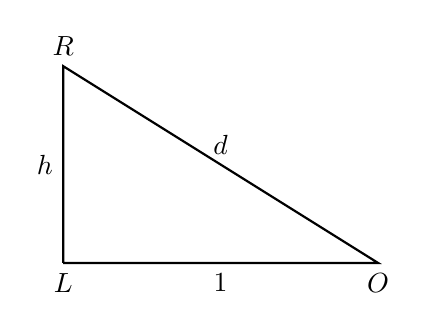
\begin{tikzpicture}[thick]
\draw (0,0)node[below]{$L$}--node[below]{1}(4,0)node[below]{$O$}--node[above]{$d$}(0,2.5)node[above]{$R$}--node[left]{$h$}(0,0);
\end{tikzpicture}
    \caption{}
\end{figure}

我们已经知道火箭的垂直高度$h$是$t$的函数$h(t)$, 又火
箭到观测站的距离$d$又是火箭的高度$h$的函数
\[d=\sqrt{1+h^2}\]
因此在时刻$t$, $R$到$O$的距离是
\[d(t)=\sqrt{1+h^2(t)}\]

上面函数$d(t)$是由$h=h(t)$和$d=f(h)=\sqrt{1+h^2}$两个函
数构成的,把其中一个函数$h(t)$代入另一个函数$f(h)$的运算
叫做复合运算,得到的函数$d(t)=f\big(h(t)\big)$叫做$t$的复合
函数。

一般说来,若$z=f(y)$, $y=g(x)$, 且$g(x)$的值域含于
$f(y)$的定义域中,那么对于$g(x)$定义域内的每一个$x$值经过
中间变数$y$, 相应地得到唯一确定的一个值$z$, 变数$z$经过
中间变数$y$而成变数$x$的函数,记为$z=f\big(g(x)\big)$, 这个函
数称为前两个函数的\textbf{复合函数}。应该指出,函数$y=g(x)$的
值域不能超出函数$f(y)$的定义域,这是极重要的。


\begin{example}
    设$z=\sqrt{1+y}$, 它的定义域$D_y=[-1,+\infty)$,
再设$y=x^2-5$, 它的定义域$D_x=(-\infty,+\infty)$, 值域$R=
[-5,+\infty)$. 

作为复合函数$z=\sqrt{1+(x^2-5)}=\sqrt{x^2-4}$,
其定义域只能是$(-\infty,-2]$和$[2,+\infty)$, 这时,$y=x^2-
5$的值域是$[-1,+\infty)$, 它没有超过$D_y=[-1,+\infty)$
的范围,这就是说复合函数$z=f\big(g(x)\big)$的定义域只能由$y=
g(x)$的定义域中那些使$g(x)$属于$z=f(y)$的定义域的$x$
组成。
\end{example}

\begin{example}
已知$f(g)=\frac{1}{g+1}$,$g=g(x)=x^2$。

求$f\big(g(x)\big)$和$g\big(f(x)\big)$。    
\end{example}

\begin{solution}
\[\begin{split}
    f\big(g(x)\big)&=\frac{1}{x^2+1}\\
    g\big(f(x)\big)&=\left(\frac{1}{x+1}\right)^2=\frac{1}{x^2+2x+1}
\end{split}\]
显然,$f\big(g(x)\big)\ne g\big(f(x)\big)$, 这表明函数的复合运算是不满足交换律的。
\end{solution}

\begin{example}
已知$f\left(\sin\frac{x}{2}\right)=\cos x+1$,
求$f\left(\cos\frac{x}{2}\right)$。
\end{example}    

\begin{solution}
    复合函数
$f\left(\sin\frac{x}{2}\right)=\cos x+1=2-2\sin^2\frac{x}{2}$
    是把函
    数$y=\sin\frac{x}{2}$
    代入$f(y)=2-2y^2$中复合而成。现在令
    $y=\cos\frac{x}{2}$代入$f(y)$,得到
\[f\left(\cos\frac{x}{2}\right)=2-2\cos^2\frac{x}{2}=2-(1+\cos x)=1-\cos x\]
\end{solution}    

在函数的运算中,我们介绍了函数的加、减、乘、除和
函数的复合五种运算,从定义来看,我们可以用上述五种运
算,由某一简单而基本的函数去造出多种多样的新函数来,
譬如从常数函数$y=c$和恒等函数$y=x$, 用加、减、乘运算就可
以得出多项式函数。其实我们常常要用到的,并不是把所给的
函数组合成更复杂的函数;而是要把所给的函数分解成更简
单的函数的组合,把要解的问题归于比较简单的问题去解决。


\begin{example}
    将函数$y=x\sin\frac{1}{x}$
分解成比较简单的函数的组
合(引进新的中间变数符号)。
\end{example}

\begin{solution}
    $y=x\sin\frac{1}{x}$
    可分解为$f(x)=x$与$g(x)=\sin\frac{1}{x}$
    之积,又$g(x)=\sin\frac{1}{x}$
    可以看作是$g(h)=\sin h$和$h=h(x)=\frac{1}{x}$
    的复合函数,于是原来的函数可以看作下面简单函数的
    组合
    \[F(x)=f(x)\cdot g\big(h(x)\big)\]
    这里$f(x)=x$, $g(h)=\sin h$, $h=h(x)=\frac{1}{x}$。    
\end{solution}

\begin{example}
求函数$\sqrt{x-\sqrt{x+1}-2}$的定义域。
\end{example}

\begin{solution}
设$F(x)=\sqrt{x-\sqrt{x+1}-2}=\sqrt{(x+1)-\sqrt{x+1}-3}$,则$F(x)$可以看作$f(y)=\sqrt{y^2-y-3}$与$y=g(x)=\sqrt{x+1}$
的复合函数,即$F(x)=f\big(g(x)\big)$且知:

$f(y)$的定义域
$D_f=\left(-\infty,\frac{1-\sqrt{13}}{2}\right]\bigcup\left[\frac{1+\sqrt{13}}{2},+\infty\right)$

$g(x)$的定义域$D_g=[-1,+\infty)$, 它的值域$R_x=[0,+\infty)$

\[\begin{split}
&\text{复合函数$F(x)=f\big(g(x)\big)$有意义}\Longleftrightarrow
\begin{cases}
    g(x)\text{有意义}\\
    g(x)\in\left[\frac{1+\sqrt{13}}{2},+\infty\right)
\end{cases}\\
&\Longleftrightarrow
\begin{cases}
    x+1\ge 0\\
    \sqrt{x+1}\ge \frac{1+\sqrt{13}}{2}
\end{cases}\Longleftrightarrow
\begin{cases}
    x\ge -1\\
    x+1\ge \left(\frac{1+\sqrt{13}}{2}\right)^2=\frac{7+\sqrt{13}}{2}
\end{cases}\\
&\Longleftrightarrow x\ge \frac{5+\sqrt{13}}{2}
\end{split}\]
$\therefore\quad $函数$\sqrt{x-\sqrt{x+1}-2}$的定义域是
$\left[\frac{5+\sqrt{13}}{2},+\infty\right)$。

如果直接求$F(x)=\sqrt{x-\sqrt{x+1}-2}$的定义域,那
么只须:
\[\begin{split}
   x-\sqrt{x+1}-2\ge 0& \Longleftrightarrow x-2\ge \sqrt{x+1} \Longleftrightarrow \begin{cases}
    x-2\ge 0\\ x+1\ge 0\\ (x-2)^2\ge (x+1)
\end{cases}\\
& \Longleftrightarrow \begin{cases}
    x\ge 2\\x\ge -1\\ x\ge \frac{5+\sqrt{13}}{2}
\end{cases} \Longleftrightarrow x\ge \frac{5+\sqrt{13}}{2}
\end{split}\]
$\therefore\quad $函数$\sqrt{x-\sqrt{x+1}-2}$的定义域是
$\left[\frac{5+\sqrt{13}}{2},+\infty\right)$。
\end{solution}

\section*{习题8.1}
\addcontentsline{toc}{subsection}{习题8.1}

试确定下面1---5里每一对函数$f$和$g$的自然定义域,并
求$f+g$, $f-g$, $f\cdot g$, $f/g$和$g/f$的相应的定义域。

\begin{enumerate}
    \item $f(x)=x,\qquad g(x)=\sqrt{x-1}$
    \item $f(x)=\frac{1}{x-2},\qquad g(x)=\frac{1}{\sqrt{x-1}}$
        \item $f(x)=\sqrt{x},\qquad g(x)=\sqrt[4]{x+1}$
    \item $f(x)=\sin x,\qquad g(x)=\cos x$
    \item $f(x)=\tan x,\qquad g(x)=\tan x$
    \item 证明函数$f(x)=\frac{1}{1+x}$在它的定义域上是单射的。又
    $x$为何值时,下列各式才有意义?
    \begin{multicols}{2}
\begin{enumerate}
    \item $f\big(f(x)\big)$
    \item $f\left(\frac{1}{x}\right)$
    \item $f(cx)$
    \item 对于哪些数$c$,有一数$x$
    能使$f(cx)=f(x)$
\end{enumerate}        
    \end{multicols}

\item 下列函数能否构成复合函数$y=f\big(\varphi(x)\big)$, 如果能够
构成,则指出复合函数的定义域和值域:
\begin{enumerate}
    \item $y=f(u)=2u+1,\qquad u=\varphi(x)=x^2$
    \item $y=f(u)=\sqrt{u},\qquad u=\varphi(x)=1-x^2$
    \item $y=f(u)=u^2+u^3, \qquad u=\varphi(x)=\begin{cases}
        1,& \text{当$x$为有理数}\\
        2,&\text{当$x$为无理数}\\
    \end{cases}$
    \item $y=f(u)=2$, 定义域为$U_1$,\qquad  $u=\varphi(x)$, 定义域为
    $X$, 值域为$U_2$。
\end{enumerate}

\item 设$f(x)=ax^2+bx+c$, 证明
$f(x+3)-3f(x+2)+3f(x+1)-f(x)=0$。
\item \begin{enumerate}
\item 设$y=f(x)=a+bx+\frac{c}{x}$, 求$f\left(\frac{2}{x}\right)$。
\item 设$y=f(x)=\sqrt{1+x+x^2}$, 求$f(x^2)$, $f(-x^2)$。
\end{enumerate}

\item 若$\varphi(x)=x^3+1$, 求$\varphi(x^2)$, $\big(\varphi(x)\big)^2$, $\varphi\big(\varphi(x)\big)$。
\item 求下列函数定义域:
\begin{multicols}{2}
 \begin{enumerate}
    \item $y=\sqrt{x}+\sqrt{-x}$
    \item $y=\sqrt[4]{\frac{(x-2)(x-3)}{x^2}}$
\end{enumerate}   
\end{multicols}

\item $a,b,c,d$取什么值,才能使函数$$f(x)=\frac{ax+b}{cx+d}$$对所有$x$满足$f\big(f(x)\big)=x$?
\end{enumerate}

\section{函数的图象}

从平面上一条曲线(对这条曲线应该要求:与纵轴平行
的直线与它的交点不能多于一个)可以引出一个函数,反过
来,给了一个函数$y=f(x)$, 那么通常采用直角坐标系,就
可以用图形来表示$y$是$x$的函数。

定义在某一变域$D$上的函数的图象就是让$x$取遍$D$中所
有值,所有点$(x,f(x))$的集合便形成平面上的一个\textbf{图形},
这个图形称为函数$y=f(x)$的\textbf{图象},而这个方程$y=f(x)$称
为\textbf{图象的方程}。

利用函数图象的几何直观可以更清楚地看出函数的一些
性质,下面我们把函数的解析性质和它的图象上相应的几何
性质对照着列出来:
\begin{center}
\begin{tabular}{cp{.45\textwidth}p{.45\textwidth}}
    \hline
    &  解析性质  &几何性质\\
    \hline
    1  &$f$是$x$的增函数,即对于任意的$a\in D$, $b\in D$, 当$a<b$时,恒有$f(a)<
f(b)$  &$f$的图象随着$x$向右移动而上升\\
2&$f$是$x$的减函数,即对于任意的$a\in D$, $b\in D$, 当$a<b$时,恒有$f(a)>f(b)$ &$f$的图象随着向右移动而下降\\
3&$f$是偶函数,即对于任意的$x\in D$, 恒有$f(-x)=f(x)$ &函数$f$的图象关于$y$轴对称\\
4& $f$是奇函数,即对于任意的$x\in D$, 恒有$f(-x)=-f(x)$ & 函数$f$的图象关于原点对称\\
5 & $f$是周期函数,即对于任意的$x\in\mathbb{R}$, 恒有$f(x+p)=f(x)$, 这里$p$是一个正的常数& 函数$f$在区间
$[0,p]$或$\left[-\frac{p}{2},\frac{p}{2}\right]$上的
图象可以沿$x$轴左、右连续推移,重复出现\\
\hline
\end{tabular}
\end{center}

下面我们给出几个常见的函数的图象。

\subsubsection{常值函数}
常值函数$f(x)=c$的图象是一条平行$x$轴的直线,它
至$x$轴的距离为$|c|$, 如图8.8。

\subsubsection{取整函数}
函数$f(x)=[x]$代表不超过$x$的最大整数,即:
若$n\le x<n+1,\; n\in\mathbb{Z}$, 则$f(x)=[x]=n$. 它的图象
如图8.9。

\begin{figure}[htp]\centering
    \begin{minipage}[t]{0.48\textwidth}
    \centering
\begin{tikzpicture}[>=latex, scale=1]
\draw[->] (-2.5,0)--(2.5,0)node[right]{$x$};
\draw[->] (0,-1)--(0,2.5)node[right]{$y$};
\draw[very thick] (-2,1.5)--(2,1.5)node[above]{$f(x)=c$};
\draw[<->] (-1,0)--node[right]{$c$}(-1,1.5);
\node at (-.25,-.25){$O$};
    \end{tikzpicture}
    \caption{}
    \end{minipage}
    \begin{minipage}[t]{0.48\textwidth}
    \centering
    \begin{tikzpicture}[>=latex, scale=1]
        \draw[->] (-2.5,0)--(3.5,0)node[right]{$x$};
        \draw[->] (0,-2.5)--(0,2.5)node[right]{$y$};
    \foreach \x in {-2,-1,1,2,3}
    {
        \draw (\x,0)node[below]{$\x$}--(\x,.1);
    }     
\foreach \x in {1,2}
{
    \draw (0,\x)node[left]{$\x$}--(.1,\x);
}
\foreach \x in {-1,-2}
{
    \draw (0,\x)--(.1,\x)node[right]{$\x$};
}

\foreach \x in {-2,-1,...,2}
{
    \draw [very thick](\x,\x)--(\x+1,\x);
    \draw (\x+1,\x)[fill=white] circle(1.5pt);
}
\node at (-.25,-.25){$O$};
    \end{tikzpicture}
    \caption{}
    \end{minipage}
    \end{figure}

\subsubsection{一次函数}

我们已经在第三册中知道,一次函数$f(x)=kx+b\; (k\ne 0)$的图象是不平行于$x$轴和$y$轴的直线。$k$称为直线的斜
率,$b$称为直线的$y$截距。若知一次函数图象上的两个点,
我们用直线方程的两点式:
\[y-y_1=\frac{y_2-y_1}{x_2-x_1}(x-x_1)\]
就可以写出一次函数的关系式。

下面给出的函数的图象是有间断点的直线:

函数$f(x)=\frac{3}{4}\cdot \frac{x^2-1}{x-1}$, 
$x\in (-\infty,1)\cup(1,+\infty)$的
图象是一条有间断点$\left(1,1\frac{1}{2}\right)$的直线,除去点$\left(1,1\frac{1}{2}\right)$外,
它与直线$y=\frac{3}{4}(x+1)$一致。(见图8.10)

\begin{figure}[htp]
    \centering
    \begin{tikzpicture}[>=latex, scale=1]
        \draw[->] (-2.5,0)--(3,0)node[right]{$x$};
        \draw[->] (0,-1)--(0,2.5)node[right]{$y$};
\foreach \x in {-1,1}
{
    \draw (\x,0)node[below]{$\x$}--(\x,.1);
}
\draw[domain=-2:2, samples=10, very thick]plot(\x, {0.75*(\x+1)});

\draw[dashed] (0,1.5)node[left]{$1\frac{1}{2}$}--(1,1.5)--(1,0);
\draw (1,1.5) [fill=white] circle(1.5pt)node[right]{$\left(1,1\tfrac{1}{2}\right)$};
\node at (2,2)[above]{$y=\frac{3}{4}(x+1)$};
        \node at (.25,-.25){$O$};
            \end{tikzpicture}    
    \caption{}
\end{figure}

\subsubsection{阶梯函数}
设点列$\{x_i\},\; i=0,1,\ldots,n$是闭区间$[a,b]$中的递增
点列,使得$x_0=a$, $x_n=b$, 即
$a=x_0<x_1<x_2<\cdots<x_{n-1}<x_n=b$,且当$x_{i-1}<x<x_i$时,
$f(x)=k_i,\; i=1,2,\ldots,n$。而$x$在分点,$x_i,\; i=0,1,\ldots,n$的
值$f(x_i)$可以任意给定,这样一个在$[a,b]$上有定义的,而
在每个子区间$(x_{i-1},x_i),\; i=1,2,\ldots,n$都是常数的函数叫
做阶梯函数。

例如,定义在$[0,6]$上的阶梯函数$f$:
\[\begin{cases}
   f(0)=2.5,\\
f(x)=2 ,&0<x\le 1,\\
f(x)=0,&1<x\le 2,\\
f(x)=-1,&2<x\le 4,\\
f(x)=2 ,&4<x\le 6. \\
\end{cases}\]
的图象如图4.11所示。

\begin{figure}[htp]\centering
    \begin{minipage}[t]{0.48\textwidth}
    \centering
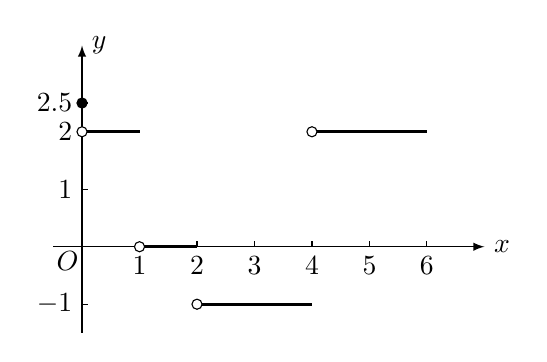
\begin{tikzpicture}[>=latex, scale=.73]
    \draw[->] (-.5,0)--(7,0)node[right]{$x$};
    \draw[->] (0,-1.5)--(0,3.5)node[right]{$y$};
\foreach \x in {1,2,...,6}
{
\draw (\x,0)node[below]{$\x$}--(\x,.1);
}
\node at (-.25,-.25){$O$};
\foreach \x in {-1,1,2,2.5}
{
\draw (0,\x)node[left]{$\x$}--(.1,\x);
}

\draw[very thick] (0,2)--(1,2);
\draw[very thick] (1,0)--(2,0);
\draw[very thick] (2,-1)--(4,-1);
\draw[very thick] (4,2)--(6,2);
\foreach \x in {{0,2},{1,0},{2,-1},{4,2}}
{
\draw (\x)[fill=white] circle(2.5pt);
}
\draw (0,2.5)[fill=black] circle(2.5pt);
    \end{tikzpicture}
    \caption{}
    \end{minipage}
    \begin{minipage}[t]{0.48\textwidth}
    \centering
    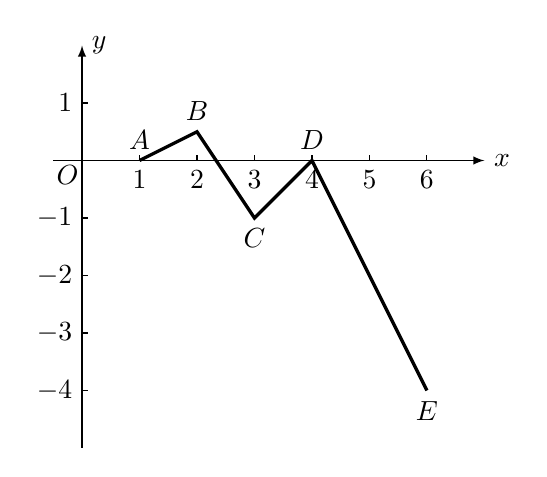
\begin{tikzpicture}[>=latex, scale=.73]
        \draw[->] (-.5,0)--(7,0)node[right]{$x$};
        \draw[->] (0,-5)--(0,2)node[right]{$y$};
\foreach \x in {1,2,...,6}
{
    \draw (\x,0)node[below]{$\x$}--(\x,.1);
}
\node at (-.25,-.25){$O$};
\foreach \x in {1,-1,-2,...,-4}
{
    \draw (0,\x)node[left]{$\x$}--(.1,\x);
}

\draw[very thick] (1,0)node[above]{$A$}--(2,.5)node[above]{$B$}--(3,-1)node[below]{$C$}--(4,0)node[above]{$D$}--(6,-4)node[below]{$E$};

    \end{tikzpicture}
    \caption{}
    \end{minipage}
    \end{figure}

\subsubsection{折线函数}
我们定义$g$:
\[g(x)=\begin{cases}
    \frac{1}{2}(x-1), & x\in[1,2]\\
    -\frac{3}{2}(x-2)+\frac{1}{2}(2-1),& x\in [2,3]\\
    (x-3)-\frac{3}{2}(3-2)+\frac{1}{2}(2-1),& x\in [3,4]\\
  -2(x-4)+(4-3)-\frac{3}{2}(3-2)+\frac{1}{2}(2-1),& x\in [4,6]\\
\end{cases}\]
它的图象是一条折线$ABCDE$, 如图4.12。


\subsubsection{幂函数}
函数$f(x)=x^n$,其中$n$为任意自然数,称为正整指数幂
函数。

为了了解正整指数幂函数的一般性质,我们在同一个坐
标系内,绘出几个这样的函数,如图4.13。

显然,当$n$为奇数时,因为$f(-x)=(-x)^n=-x^n=-f(x)$,
所以函数是奇函数。又所有正整指数幂函数,当$x=0$时,
$f(0)=0$。故每个奇次幂函数的图象通过原点,位于第一和
第三象限内且关于原点对称。所有这样的函数都是增函数。

当$n$为偶数时,因为$f(-x)=(-x)^n=x^n=f(x)$,所以
函数是偶函数,每个图象通过原点,位于第一和第二象限内
且关于$y$轴对称。

由于当$x=1$时,$f(1)=1^n=1$, 每个正整指数幂函数的
图象都通过点$(1,1)$。

\begin{figure}[htp]
    \centering
    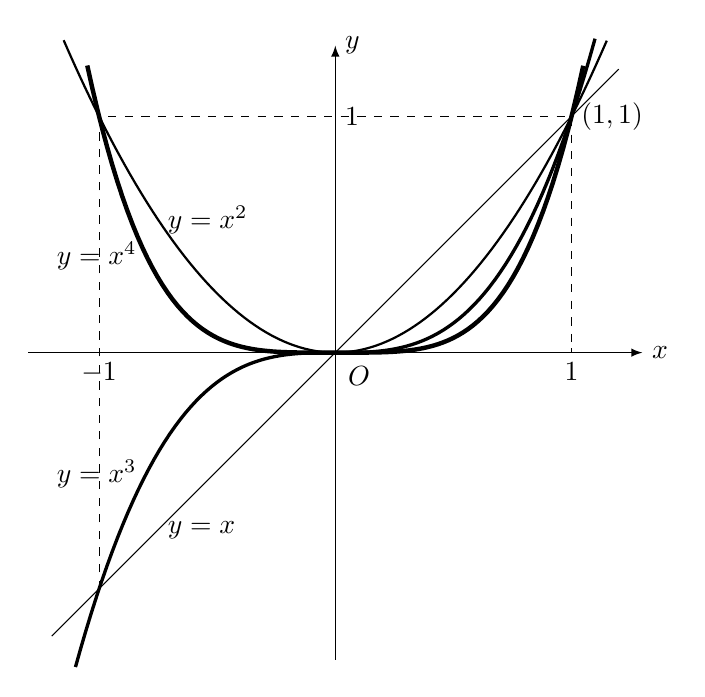
\begin{tikzpicture}[>=latex, scale=3]
        \draw[->] (-1.3,0)--(1.3,0)node[right]{$x$};
        \draw[->] (0,-1.3)--(0,1.3)node[right]{$y$};
\foreach \x in {-1,1}
{
    \draw (\x,0)node[below]{$\x$}--(\x,.02);
}
\node at (.1,-.1){$O$};
\draw[dashed](-1,-1)--(-1,1)--(1,1)--(1,0);

\draw (-1.2,-1.2)--(1.2,1.2);
\draw [domain=-1.15:1.15, samples=100, thick]plot(\x, {\x*\x});
\draw [domain=-1.1:1.1, samples=100, very thick]plot(\x, {\x*\x*\x});
\draw [domain=-1.05:1.05, samples=100, ultra thick]plot(\x, {\x*\x*\x*\x});
\node at (0,1)[right]{1};
\node at (1,1)[right]{$(1,1)$};
\node at (-.75,-.75)[right]{$y=x$};
\node at (-.8,-.512)[left]{$y=x^3$};
\node at (-.75,.5625)[right]{$y=x^2$};
\node at (-.8,.41)[left]{$y=x^4$};
            \end{tikzpicture}    
    \caption{}
\end{figure}

现在让指数$n$逐次增大,看看图象的变化,从图8.14,
8.15可以清楚地看出每个图象的平坦部分和陡峭部分,曲线
最终以图8.14和8.15中的粗黑线为极限位置。

函数$f(x)=x^{-n}$($x\ne 0$, $n$为自然数)称为负整指数幂函数。
在同一坐标系内,绘出$y=x^{-1}$, $y=x^{-2}$, $y=x^{-3}$, $y=x^{-4}$
的图象如图8.16所示。当$x=0$时,这些函数都无意义,函数
的图象在此点断开,它的二支以$y$轴为渐近线。

当指数为负奇数时,这些函数是奇函数。图象的二支分
别位于第一和第三象限内,随$x$向右移动下降,且关于原点
对称。因此,函数在$(-\infty,0)$或$(0,+\infty)$内是减函数。

当指数是负偶数时,这些函数是偶函数,每个函数的图
象在原点处断开,分为二支,位于第一和第二象限内,都以
$y$轴为渐近线,且关于$y$轴对称。从图象明 显地看出,当
$x<0$时,函数是增函数,当$x>0$时,函数是减函数。

下面我们来说明一些函数的图象如何由另一些函数的已
知图象经过某些几何变换得到。

若对于任意的$x\in D$, 函数$f$和$g$满足$g(x)=f(x-c)$,
这里$c$是常数,则若$c>0\; (c<0)$,$y=g(x)$的图象可以由
$y=f(x)$的图象,平行$x$轴右移(或左移)$|c|$个单位得到。

若函数$f$和$g$满足等式$g(x)=f(kx)$, 这里$k$是常数,则若
$k>1\; (0<k<1)$, $y=g(x)$的图象可以由$y=f(x)$的图象经
过把它上面的所有点的横坐标垂直于$y$轴压缩(或拉长)倍
而纵坐标不变的几何变换得到。

若函数$f$和$g$满足等式,$g(x)=kf(x)$, 这里$k$是常数,
则若$k>1\; (0<k<1)$, $y=g(x)$的图象可以由$y=f(x)$的图
象经过把它上面的所有点的纵坐标垂直$x$轴拉长(或压缩)
$k$倍而使横坐标不变的几何变换得到。

下面我们用例子说明图象的几何变换。
\begin{figure}[htp]\centering
    \begin{minipage}[t]{0.48\textwidth}
    \centering
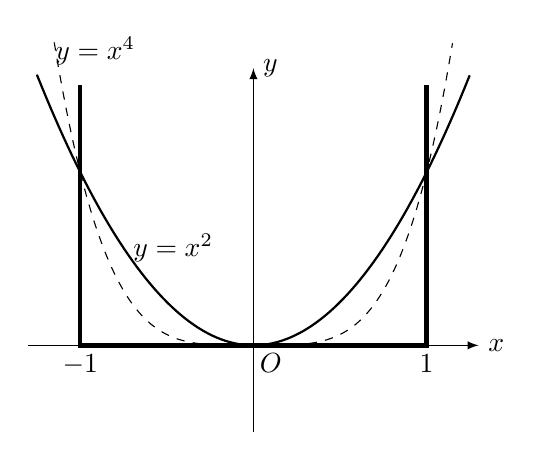
\begin{tikzpicture}[>=latex, scale=2.2]
    \draw[->] (-1.3,0)--(1.3,0)node[right]{$x$};
    \draw[->] (0,-.5)--(0,1.6)node[right]{$y$};
\foreach \x in {-1,1}
{
\draw (\x,0)node[below]{$\x$}--(\x,.02);
}
\node at (.1,-.1){$O$};
\draw[ultra thick](-1,1.5)--(-1,0)--(1,0)--(1,1.5);
\draw [domain=-1.25:1.25, samples=100, thick]plot(\x, {\x*\x});
\draw [domain=-1.15:1.15, samples=100, dashed]plot(\x, {\x*\x*\x*\x});
\node at (-.75,.5625)[right]{$y=x^2$};
\node at (-1.2,1.7)[right]{$y=x^4$};      
    \end{tikzpicture}
    \caption{}
    \end{minipage}
    \begin{minipage}[t]{0.48\textwidth}
    \centering
    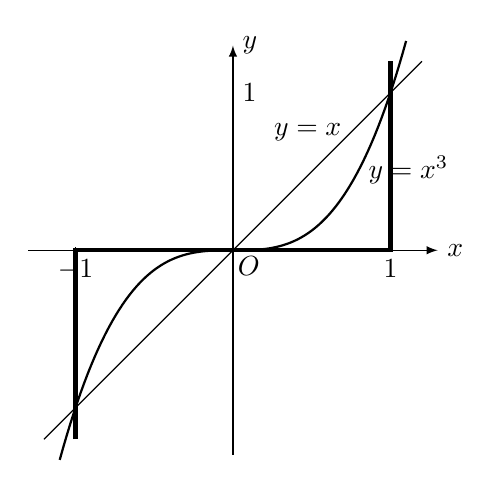
\begin{tikzpicture}[>=latex, scale=2]
        \draw[->] (-1.3,0)--(1.3,0)node[right]{$x$};
        \draw[->] (0,-1.3)--(0,1.3)node[right]{$y$};
\foreach \x in {-1,1}
{
    \draw (\x,0)node[below]{$\x$}--(\x,.02);
}
\node at (.1,-.1){$O$};
\draw[ultra thick](-1,-1.2)--(-1,0)--(1,0)--(1,1.2);
\draw (-1.2,-1.2)--(1.2,1.2);
\draw [domain=-1.1:1.1, samples=100, thick]plot(\x, {\x*\x*\x});
\node at (0,1)[right]{1};
\node at (.75,.75)[left]{$y=x$};
\node at (.8,.512)[right]{$y=x^3$};
    \end{tikzpicture}
    \caption{}
    \end{minipage}
    \end{figure}

\begin{figure}[htp]
    \centering
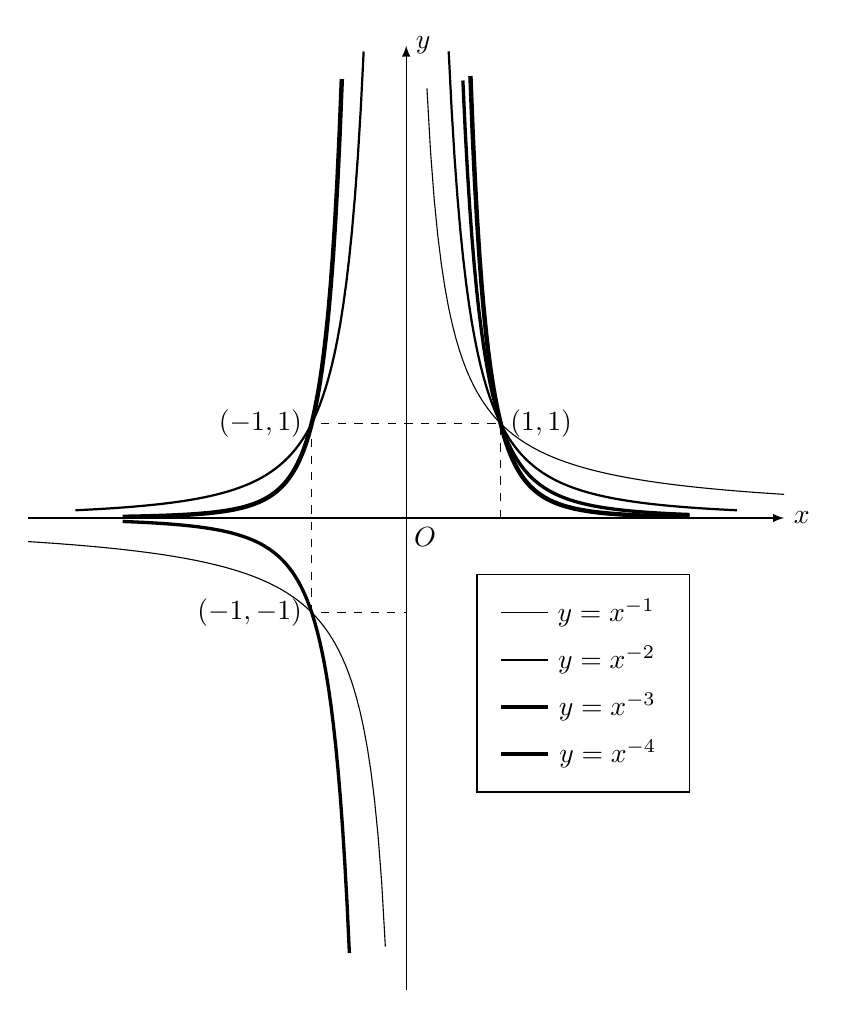
\begin{tikzpicture}[>=latex, scale=1.2]
    \draw[->] (-4,0)--(4,0)node[right]{$x$};
    \draw[->] (0,-5)--(0,5)node[right]{$y$};
\draw [domain=-4:-.22, samples=100]plot(\x, {1/\x});
\draw [domain=-3.5:-.45, samples=100, thick]plot(\x, {1/(\x*\x)});
\draw [domain=-3:-.6, samples=100, very thick]plot(\x, {1/(\x*\x*\x)});
\draw [domain=-3:-.68, samples=100, ultra thick]plot(\x, {1/(\x*\x*\x*\x)});  
\node at (.2,-.2){$O$};
\draw [domain=.22:4, samples=100]plot(\x, {1/\x});
\draw [domain=.45:3.5, samples=100, thick]plot(\x, {1/(\x*\x)});
\draw [domain=.6:3, samples=100, very thick]plot(\x, {1/(\x*\x*\x)});
\draw [domain=.68:3, samples=100, ultra thick]plot(\x, {1/(\x*\x*\x*\x)});  

\draw[dashed](1,0)--(1,1)node[right]{$(1,1)$}--(-1,1)node[left]{$(-1,1)$}--(-1,-1)node[left]{$(-1,-1)$}--(0,-1);

\draw (1,-1)--(1.5,-1)node[right]{$y=x^{-1}$};
\draw[thick] (1,-1.5)--(1.5,-1.5)node[right]{$y=x^{-2}$};
\draw[very thick]  (1,-2)--(1.5,-2)node[right]{$y=x^{-3}$};
\draw[ultra thick]  (1,-2.5)--(1.5,-2.5)node[right]{$y=x^{-4}$};
\draw (.75,-.6) rectangle (3,-2.9);


\end{tikzpicture}
    \caption{}
\end{figure}



\begin{example}
    说明$y=f(x)=\sin x$和$y=g(x)=\cos x$的图象的
关系。
\end{example}


\begin{solution}
 这两个函数的定义域都是$(-\infty,+\infty)$,根据$f(x)=
\sin x$和$g(x)=\cos x$是周期等于$2\pi$的函数,因此我们可以先在
长度等于$2\pi$的区间上来讨论这两个函数。

设$f(x)=\sin x$的定义域$D_y=[0,2\pi]$, 因为余弦函数
$g(x)=\cos x$可以看作正弦函数$\sin x$ 与$x'=x+\frac{\pi}{2}$
的复合函数,即$g(x)=\cos x=\sin\left(x+\frac{\pi}{2}\right)$,
所以复合函数$\sin\left(x+\frac{\pi}{2} \right)$
有意义,必须且只须$0\le x+\frac{\pi}{2}\le 2\pi$,
由此得到$-\frac{\pi}{2}\le x\le \frac{3\pi}{2}$。

这就是说$y=g(x)=\cos x$ 的定义域是
$D_g=\left[-\frac{\pi}{2},\frac{3\pi}{2}\right]$。
因为区间$D_g$是把区间$D_f$左移了$\frac{\pi}{2}$
个单位的结果,并且对于$D_g=\left[-\frac{\pi}{2},\frac{3\pi}{2}\right]$中
的每一个$x$都可以在$D_f=[0,2\pi ]$中找
到相应的$x+\frac{\pi}{2}$
使得
$\cos x=\sin\left(x+\frac{\pi}{2}\right)$,
所以$y=\sin x$在
区间$D_f=[0,2\pi]$ 上的一段图象左移
$\frac{\pi}{2}$个单位就得到$y=\cos x$在区间$D_g=
\left[-\frac{\pi}{2},\frac{3\pi}{2}\right]$上
的一段,因此,将$y=\sin x$的整个图象左移$\frac{\pi}{2}$
个单位就得到整个$y=\cos x$的图象了,如图
8.17所示。
\begin{figure}[htp]
    \centering
\begin{tikzpicture}[>=latex, scale=.8]
    \draw[->] (-5.5,0)--(9,0)node[right]{$x$};
    \draw[->] (0,-2)--(0,2)node[right]{$y$};
    \foreach \x/\xtext in {-3/-\tfrac{3\pi}{2},-1/-\tfrac{\pi}{2},1/\tfrac{\pi}{2},3/\tfrac{3\pi}{2},5/\tfrac{5\pi}{2}}
    {
        \draw(\x*pi/2, 0)node[below]{$\xtext$}--(\x*pi/2,.2);
    }
    \foreach \x/\xtext in {-1/-\pi, 1/\pi, 2/2\pi}
    {
        \draw(\x*pi, 0)--(\x*pi,.2)node[above]{$\xtext$};
    }
    \draw [domain=-pi:2.5*pi, samples=100, very thick]plot(\x, {cos(\x r)});
    \draw [domain=-1.5*pi:2.5*pi, samples=100,  thick]plot(\x, {sin(\x r)});
    \node at (.4,-.4){$O$};
 \node at (-pi,-1)[below]{$y=\cos x$};
 \node at (2.5*pi,1)[right]{$y=\sin x$};
\end{tikzpicture}    
    \caption{}
\end{figure}

$\because\quad \sin(-x)=-\sin x,\qquad \therefore\quad y=\sin x$的图象关于原点对称。

$\because\quad \cos(-x)=\cos x,\qquad \therefore\quad y=\cos x$的图象关于$y$轴对称。

\end{solution}

\begin{example}
    说明函数$y=f(x)=\sqrt{1-x^2}$, $D_f=[-1,1]$和
    $y=g(x)=\sqrt{1-4x^2}$的图象的关系。
\end{example}

\begin{solution}
    我们已经知道$f$的定义域是$D_f=[-1,1]$且$g(x)$可
以看作$f(x')$与$x'=2x$的复合函数,即
\[g(x)=f(2x)=\sqrt{1-(2x)^2}\]

复合函数$f(2x)$有意义必须且只须$-1\le 2x\le 1$, 即:
\[-\frac{1}{2}\le x\le \frac{1}{2}\]
因此,$g(x)$的定义域是$D_g=\left[-\frac{1}{2},\frac{1}{2}\right]$。
因为对于$D_g=\left[-\frac{1}{2},\frac{1}{2}\right]$中
的每一个$x$, 在$D_f$中一定有一个相应的$2x$使
得$g(x)=f(2x)$成立,这就说明了将$y=f(x)$的图象上所有
点的横坐标垂直$y$轴压缩一半而使点的纵坐标不变便得
$g(x)=\sqrt{1-4x^2}$的图象,如图4.18所示。

\begin{figure}[htp]
    \centering
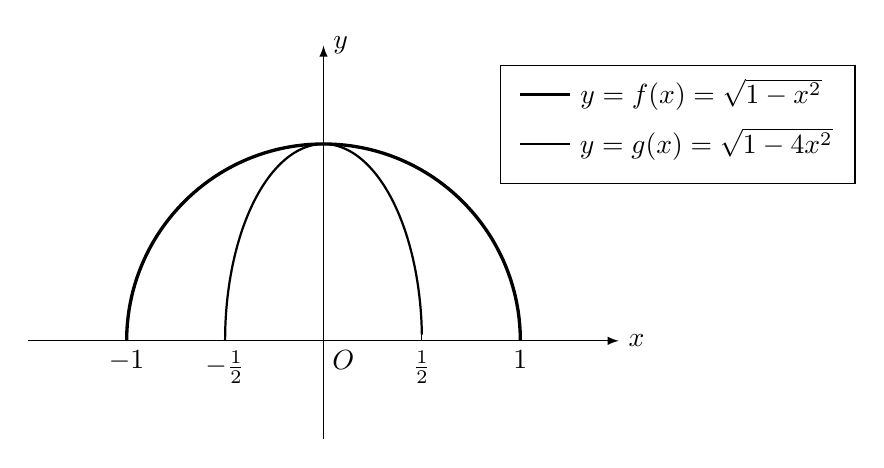
\begin{tikzpicture}[>=latex, scale=2.5]
    \draw[->] (-1.5,0)--(1.5,0)node[right]{$x$};
    \draw[->] (0,-.5)--(0,1.5)node[right]{$y$};
\draw [very thick](-1,0) arc (180:0:1);
\draw[domain=-.5:.5, samples=1000, thick] plot(\x, {sqrt(1-4*\x*\x)});
\foreach \x/\xtext in {-1/-1,-.5/-\frac{1}{2},.5/\frac{1}{2},1/1}
{
    \draw (\x,0)node[below]{$\xtext$}--(\x,.1);
}
\node at (.1,-.1){$O$};

\draw[thick] (1,1)--(1.25,1)node[right]{$y=g(x)=\sqrt{1-4x^2}$};
\draw[very thick] (1,1.25)--(1.25,1.25)node[right]{$y=f(x)=\sqrt{1-x^2}$};
\draw (.9,.8) rectangle (2.7,1.4);
\end{tikzpicture}
    \caption{}
\end{figure}
\end{solution}

\begin{ex}
\begin{enumerate}
    \item 试由函数增减性的定义,说明下面函数的增减性:
    \begin{multicols}{2}
\begin{enumerate}
    \item $y=x^3$
    \item $y=x^{-2}$
    \item $f(x)=\sqrt{x}$
    \item $g(x)=\sqrt[3]{x}$
    \item $h(x)=\frac{1}{\sqrt{x}}$
\end{enumerate}        
    \end{multicols}

    \item 作下列函数的图象:
    \begin{multicols}{2}
        \begin{enumerate}   
\item $y=\sqrt{x}$
\item $y=x-[x]$
\item $y=\sqrt{x-[x]}$
\item $y=[x]+\sqrt{x-[x]}  $
        \end{enumerate}        
    \end{multicols}
    \item 若一折线函数的图象$ABCDE$的顶点坐标是
\[A\left(-1,-1\frac{1}{2}\right),\quad B(1,1),\quad C(3,-1),\quad D(6,2.5),\quad E(7,2.5)\]    
写出这个函数的解析式。

\item 作下列函数的图象:
\begin{multicols}{2}
    \begin{enumerate}  
\item $f(x)=|2x|$
\item $f(x)=\frac{|x|}{x}$
\item $y=|4-x^2|,\quad -3\le x\le 3$
\item $y=|x^2-2x-3|$
\end{enumerate}        
\end{multicols}
\item 已知点$P(\alpha,\beta)$和一水平线$L$即$g(x)=\gamma$的图象。证
明至$P$与$L$等距离的所有点$(x,y)$的集合,是具有$f(x)=
ax^2+bx+c$形式的函数的图象。
\end{enumerate}
\end{ex}

\section{函数的连续性}
在初中一年级讨论平方根时,我们曾用下面的想法初步
地肯定$\sqrt{2}$的“存在性”:边长是1米的正方形面积是1平
方米;边长是2米的正方形面积是4平方米,所以,当一个正
方形的边长逐渐增加时,它的面积逐渐由1平方米增加到4
平方米,中间应该会有那么一个2平方米的正方形。

上面这段话只是一个粗略的想法,用数学语言来表达
如下:

$y=f(x)=x^2$, 这个幂函数的函数值,在$x=1$时,$f(1)=1^2=1$;
$x=2$时,$f(2)=2^2=4$; 当$x$由1变到2时,$x$的值应
该由1“连续地”变到4, 所以$x$应该能取一个值$x_0$使
$f(x_0)=x^2_0=2$。

上面说的“连续地”这个术语究竟是什么意思呢?在这
一节中,我们就是要把“连续性”的涵意加以分析、确立。
并且,把上面这个粗略的想法体现成一个明确有用的定
理——中间值定理。

\subsection{连续函数的概念}
从几何的直观来看,连续与间断的意思是一目了然的,
一条曲线是连续的,指这条曲线没有间断点,在上一节考察
的函数,展示了函数图象有间断点的情形,函数$f$在点$x_0$是
否连续只依赖于它在$x_0$的一个(任意小的)邻域内的变化情
况。直观地看来,如果
\begin{enumerate}
\item $f$在其定义域的点$x_0$的邻域$(x_0-\delta,x_0+\delta)$内
有定义;
\item 当$x$充分接近$x_0$时,函数值$f(x)$同$f(x_0)$相差任
意小,即自变量$x$的微小变化只能引起函数值的微小变化,
从而排除了函数值的跳跃,就函数的图象来看,在这一点
$x_0$的邻近,函数图象是由一条曲线组成的,而没有在这一点
断开成为两个分支,那么称函数$f$在点$x_0$连续。
\end{enumerate}


“充分接近”和“相差任意小”这两句话是不够明确的,而
必须用定量的术语给以严格的表述。现在我们可以用数列极
限的概念把“当$x$充分接近$x_0$时,$f(x)$与$f(x_0)$相差任意小”
这句话定量地描述如下:

如果在函数定义域$I$中,自变量$x$取任何一个收敛于$x_0\in I$
(即$\displaystyle\lim_{i\to\infty}x_i=x_0$)的数列$\{x_i\}$的项$x_i\; (i=1,2,\ldots)$, 那么对应
的函数数列:
\[f(x_1),\; f(x_2),\; \ldots,\;  f(x_i),\ldots\]
总有极限值$f(x_0)$, 即
\[\lim_{i\to\infty} f(x_i)=f(x_0)\]

于是我们得到下述连续性的严格定义:

\begin{blk}{定义}
     定义在区间$I$上的一个函数$f$在点$a\in I$称做连
续,如果
\begin{enumerate}
\item $f(a)$有一个确定值,
\item 对于$I$中每一个收敛于$a$的数列$\{x_i\}$, 对应的函数
数列$\{f(x_i)\}$总以$f(a)$为极限,即有关系式:
$\displaystyle\lim_{i\to \infty}f(x_i)=f(a)=f\left(\displaystyle\lim_{i\to \infty}x_i\right)$
成立。
\end{enumerate}
\end{blk}


这个定义表明对于一个连续函数$f$, 记号lim可以和记号
$f$互换。

我们举几个例子说明如何用这个定义来验证函数$f$在点
$a$处连续或间断。


\begin{example}
    函数$f(x)=\frac{3}{4}\cdot\frac{x^2-1}{x-1}$
在点$x=1$处不连续,因为
$f(1)$没有意义。
\end{example}

\begin{example}
    函数$f(x)=[x]$在整数点$n$处不连续,因为当
$x=n,\; (n\in\mathbb{Z})$时,函数$f(x)=[x]$有确定值$f(n)=[n]=n$。
虽然当$x$取的数列$\{x_i\}$的值,从$x=n$的右边趋于$n$时,
有$\Lim_{i\to\infty}f(x_i)=\Lim_{i\to\infty}[x_i]=n=f(n)$, 但是当$x$取的数列$\{x'_n\}$从$x=n$的左边趋于$n$时,即当$x'_i$满足条件:$n-1\le x'_i <m$, $\Lim_{i\to \infty}x'_i=n$时,那么
\[\Lim_{i\to \infty}f(x'_i)=\Lim_{i\to \infty}[x'_n]=n-1\ne f(n)=n\]
这就是说$f(x)=[x]$的图象是在整数点具有跳跃性间断的
曲线。
\end{example}

现在我们来考虑另一种间断性的曲线。
\begin{example}
    函数$f(x)=\frac{1}{x}$
    在点$x=0$处不连续,因为$f(0)$不
    存在,并且任何数列$\{x_i\}$收敛于0时,例如:
    
    当$x_i>0$, $x_i\to 0$时,即$x_i$从右边趋近于原点时,有
$\Lim_{i\to\infty}\frac{1}{x_i}=+\infty$;

    当$x_i<0$, $x_i\to 0$时,即$x_i$从左边趋近于原点时,有
    $\Lim_{i\to\infty}\frac{1}{x_i}=-\infty$;

    当$\{x_i\}$是任意一个趋于0的数列时,则$\Lim_{i\to\infty}\left|\frac{1}{x_i}\right|=\infty$。

    无论哪种情形,数列$\left\{\frac{1}{x_i}\right\}$
    趋向无穷大。
\end{example}

\begin{rmk}
例8.16和例8.18的分母的零点都是函数的不连续点,
但是例8.16中的分式:$f(x)=\frac{3}{4}\cdot\frac{x^2-1}{x-1}$,
当$x=1$时,代数恒等式
\[\frac{3}{4}\cdot\frac{x^2-1}{x-1}=\frac{3}{4}(x+1)\]
是成立的。因此任何数列$x_i\; (\ne 1)$趋于1时,由于$x_i\ne 1$,
\[\begin{split}
    \Lim_{i\to\infty}f(x_i)&=\Lim_{i\to\infty}\frac{3}{4}\cdot \frac{x^2_i-1}{x_i-1}=\Lim_{i\to\infty}\frac{3}{4}(x_i+1)\\
    &=\frac{3}{4}(1+1)=\frac{3}{2}
\end{split}\]

这就是说,对于任何收敛于1的数列$\{x_i\}$, 对应的函数数
列$\{f(x_i)\}$都以$\frac{3}{2}$为极限。 

如果我们定义一个新函数$F$:
\[F(x)=\begin{cases}
    \frac{3}{4}\cdot\frac{x^2-1}{x-1},& x\ne 1\\
    \frac{3}{2}, & x=1
\end{cases}\]
那么$F(x)$在点$x=1$处就连续了。
\end{rmk}

\begin{blk}{定义}
     如果对于任何收敛于$a$的数列$\{x_i\}$, $\Lim_{i\to\infty}f(x_i)$存在,并且彼此相等,但不等于$f(a)$, 或者$f(a)$没有定义,则
称$f$在$a$处有可去间断点。
\end{blk}

例8.16中的$x=1$就是$f$的可去间断点。

\begin{blk}{定义}
    如果函数$f$在定义域$I$中每一点都连续,就说$f$
是$I$上的一个连续函数,或简称为连续函数。
\end{blk}

\subsection{连续函数的运算}
由连续函数定义知道,函数$f$在$a\in I$连续当且仅当:若
$I$里的每个数列$\{x_i\}$收敛于$a$时,数列$\{f(x_i)\}$也收敛于
$f(a)$。

我们可以把上述条件:
\[\lim_{i\to \infty}x_i=a \quad \Longrightarrow\quad \lim_{i\to \infty}f(x_i)=f(a)\]
简写成:
\[\lim_{x\to a}f(x)=f(a)=f\left(\lim_{x\to a}x\right)\]

由数列极限运算定理直接得出下面定理。

\begin{blk}{定理1}
    设$f$和$g$在$a$处连续,即
    \[\lim_{x\to a}f(x)=f(a),\qquad \lim_{x\to a}g(x)=g(a)\]
    则
\begin{enumerate}
    \item $\Lim_{x\to a}[f(x)\pm g(x)]=f(a)\pm g(a)$,(即$f\pm g$在$a$处连续)。
    \item $\Lim_{x\to a}f(x)\cdot g(x)=f(a)\cdot g(a)$,(即$f\cdot g$在$a$处连续)。
    \item 若$g(a)\ne 0$,$\Lim_{x\to a}\frac{1}{g(x)}=\frac{1}{g(a)}$,(即$1/g$在$a$处连续)。
\end{enumerate}
\end{blk}

\begin{example}
    函数$f(x)=x^k$ ($k$是一个正整数,$x\in\mathbb{R}$) 到处连
续,即$\Lim_{x\to a}x^k=a^k,\; (a\in\mathbb{R})$。
\end{example}

\begin{proof}
对$k$用数学归纳法来证明,设$a$是$f$的定义域$\mathbb{R}$
中任何一点。

当$k=1$时,显然,$\Lim_{x\to a}x=a$, 命题成立。

假设当$k=i\; (i\in\mathbb{N})$时,有
\[\Lim_{x\to a} x^i=a^i\qquad (i\in\mathbb{N})\]
那么,当$k=i+1$时,有
\[\Lim_{x\to a}x^{i+1}=\Lim_{x\to a} x^i\cdot x=\Lim_{x\to a} x^i\cdot \Lim_{x\to a} x=a^i\cdot a=a^{i+1}\]    
于是,对于所有正整数$k$, $f(x)=x$在任何一点$a$连续,也
即$f(x)=x$到处连续。
\end{proof}


由定理1和$f(x)=x^k\; (k\in\mathbb{N})$, 及常数函数$g(x)=c$ ($c$是常数)的到处连续性,我们可以证明下面的命题
成立。

\begin{blk}{命题1}
    任何多项式函数到处连续。
\end{blk}

进一步推得下面命题:

\begin{blk}{命题2}
    若$f$和$g$是两个多项式,$g\ne 0$, 那么有理函
数$r=f/g$,
除去$g$的零点集合,函数$r$是有定义的而且是
连续的。
\end{blk}

\begin{blk}{命题3}
    $f(x)=\sqrt[n]{x}$在区间$(0,+\infty)$上连续,即 
\[\lim_{x\to x_0}\sqrt[n]{x}=\sqrt[n]{x_0}\qquad (x\in[0,+\infty))\]
\end{blk}

\begin{proof}
    设$x_0$是一个任给正数,数列$\{x_i\}$是在$[0,+\infty)$
内任何一个收敛到$x_0$的数列,即$\Lim_{i\to \infty} x_i=x_0$。我们要证明,当
$\Lim_{i\to\infty} x_i=x_0$时,$\Lim_{i\to\infty} (\sqrt[n]{x_i}-\sqrt[n]{x_0})=0$。

在代数恒等式:
\[(A-B)\left(A^{n-1}+A^{n-2}B+\cdots +AB^{n-2}+B^{n-1}\right)=A^n-B^n\]
中,以$A=x_i^{\tfrac{1}{n}}$, $B=x_0^{\tfrac{1}{n}}$代入,即得:
\begin{equation}
\sqrt[n]{x_i}-\sqrt[n]{x_0}=\frac{x_i-x_0}{x_i^{\tfrac{n-1}{n}}+x^{\tfrac{n-2}{n}}_i\cdot x_0^{\tfrac{1}{n}}+\cdots +x^{\tfrac{1}{n}}_i\cdot x_0^{\tfrac{n-2}{n}} + x_0^{\tfrac{n-1}{n}}} 
\end{equation}
由于$\Lim_{i\to\infty}x_i=x_0$, 根据数列极限定义,取
$\varepsilon=\frac{x_0}{2}$,
则存在正整数$N$, 使得当$i>N$时,有
\[x_i>x_0-\frac{x_0}{2}=\frac{x_0}{2}\]
从而,当$i>N$时,有
\begin{equation}
    (x_i)^{\tfrac{1}{n}}=\left(\frac{x_0}{2}\right)^{\tfrac{1}{n}}
\end{equation}
此外,显然有
\begin{equation}
    (x_0)^{\tfrac{1}{n}}=\left(\frac{x_0}{2}\right)^{\tfrac{1}{n}}
\end{equation}

由(8.2)---(8.4)立即得
\[\left|\sqrt[n]{x_i}-\sqrt[n]{x_0}\right|<\frac{|x_i-x_0|}{n\left(\sqrt[n]{\frac{x_0}{2}}\right)^{n-1}}\]
当$i\to\infty$时,$|x_i-x0|\to 0$, 又因为$n\left(\sqrt[n]{\frac{x_0}{2}}\right)^{n-1}$
是一个和$i$
无关的常数,所以
\[\left|\sqrt[n]{x_i}-\sqrt[n]{x_0}\right|\to 0\]
即
\[\lim_{x\to x_0} \sqrt[n]{x}=\sqrt[n]{x_0}\]
这也就证明了$f(x)=\sqrt[n]{x}$ 在区间$[0,\infty)$上到处连续。
\end{proof}

我们在这里介绍了函数连续性的严格定义,对于初学者
只要能够正确理解这一分析定义的涵义就可以了,以后在第
六册微积分中,我们还要对它进行研究。

\subsection{连续函数的中间值定理}
平面上一个一目了然的性质是:一条直线把平面分割成
两半,例如,在$(x,y)$坐标平面上,直线$y=c$就把平
面分成$y<c$和$y>c$这两半,从上半平面走到下半平面的
连续通路,必须和分界线$y=c$相交,下述中间值定理也就
是上述直观现象的代数化:

\subsubsection{中间值定理}

设$y=f(x)$是一个在闭区间$[a,b]$
上到处连续的函数,设$c$是一个介于$f(a)$和$f(b)$之
间的常数,则必存在一个介于$a,b$之间的实数$x_0$, 使得
$f(x_0)=c$。用几何术语来说:$y=f(x)$, $a\le x\le b$的图象
是一条还结$P(a,f(a))$点和$Q(b,f(b))$点的连
续曲线,而$P,Q$分居于直线$y=c$的两侧,则曲线$y=
f(x),\; a\le x\le b$至少和直线$y=c$有一个交点$(x_0,
f(x_0)=c)$,(图8.19)。

\begin{figure}[htp]
    \centering
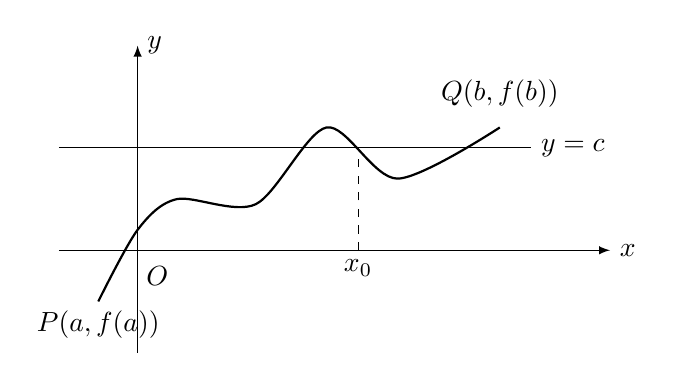
\begin{tikzpicture}[>=latex, yscale=1.3]
    \draw[->] (-1,0)--(6,0)node[right]{$x$};
    \draw[->] (0,-1)--(0,2)node[right]{$y$};
    \draw(-1,1)--(5,1)node[right]{$y=c$};
    \node at (.25,-.25){$O$};
    \draw[ thick] plot[smooth] coordinates{(-.5,-.5)(0,.2) (.5,.5) (1.5,.45) (2.4,1.2)(3.3,.7)(4.6,1.2)};
\node at (-.5,-.5)[below]{$P(a,f(a))$};
\node at (4.6,1.3)[above]{$Q(b,f(b))$};
\draw[dashed] (2.8,0)node[below]{$x_0$}--(2.8,1);
\end{tikzpicture}
    \caption{}
\end{figure}


在给出这个定理的证明之前,我们先讨论一个特例,让
$f(x)=x^3+x-3$, $a=1$, $b=2$. 由于$f(1)=-1$与$f(2)=7$异号,我们将说明在1,
2之间一定存在$f(x)=x^3+x-3$的根$k$, 使$f(k)=0$。

从$y=x^3+x-3$的图象
(图8.20)上看,这个命题是一
目了然的,现在我们要把二分
逼近法与实数完备性,函数连
续性配合一起来说明它的根的
存在和根的求法。

\begin{figure}[htp]
    \centering
\begin{tikzpicture}[>=latex, yscale=.6]
\draw[->] (-2,0)--(3,0)node[right]{$x$};
\draw[->] (0,-9)--(0,8)node[right]{$y$};
\foreach \x in {-8,-7,...,-1,1,2,...,7}
{
    \draw (-.1,\x) node[left]{$\x$} --(0,\x);
}
\node at (.4,-.4){$O$};
\draw[domain=-1.6:2, samples=100, very thick] plot(\x, {\x*\x*\x+\x-3});
\node at (2,5)[right]{$y=x^3+x-3$};
\end{tikzpicture}
    \caption{}
\end{figure}


首先,我们容易验证这个
方程没有整数根$\pm 1$和$\pm 3$, 
因此所求的根一定是一个无理
数,由于闭区间$[a,b]=
[1,2]$具有性质$P:f(a)\cdot f(b)<0$, 即$f(a)$与
$f(b)$异号。当我们把它二
等分时,至少会有一个分段保
有这个性质$P$, 照这样,不断地二等分保有性质$P$的分段,
我们就可以得到保有性质$P$的两串左、右夹逼数列如下:

令$x=\frac{1+2}{2}=\frac{3}{2}$, 
显然$f\left(\frac{3}{2}\right)\ne 0$, 否则$f(x)$就
会有有理数根$\frac{3}{2}$,
无论$f\left(\frac{3}{2}\right)$是正还是负,在$\left[1,\frac{3}{2}\right]$和$\left[\frac{3}{2},2\right]$
这两个分段中一定有一段具有性质$P$, 算出
\[f\left(\frac{3}{2}\right)=\frac{3}{8}>0\]

取$a_1=1$, $b_1=\frac{3}{2}$, 
闭区间$[a_1,b_1]=\left[1,\frac{3}{2}\right]$
保有性质$P$, 照这样进行有限次后,由于$f(x)$没有有理根,
所以$f\left(\frac{a_m+b_m}{2}\right)\ne 0$, 这就使我们每次由$[a_m,b_m]$选取保
有性质$P$的一个分段$[a_{m+1},b_{m+1}]$之后,还可以细分下去,
因此,这个过程是无终止的。
\begin{itemize}
\item 令$x=\frac{a_1+b_1}{2}=\frac{1+\frac{3}{2}}{2}=\frac{5}{4}$,算出$f\left(\frac{5}{4}\right)=\frac{13}{64}>0$,取$[a_2,b_2]=\left[1,\frac{5}{4}\right]$;
\item 
令$x=\frac{a_2+b_2}{2}=\frac{1+1.25}{2}=1.125$, 算出$f\left(1.125\right)=-0.4512<0$,取$[a_3,b_3]=\left[1.125,1.25\right]$;
\item 
令$x=\frac{a_3+b_3}{2}=\frac{1.125+1.25}{2}=1.1875$, 算出$f\left(1.1875\right)=-0.1379<0$,取$[a_3,b_3]=\left[1.1875,1.25\right]$;
\item 
令$x=\frac{1.1875+1.25}{2}=1.2188$, 算出$f\left(1.2188\right)=0.029>0$,取$[a_4,b_4]=\left[1.1875,1.2188\right]$;

\item 
令$x=\frac{1.1875+1.2188}{2}=1.203$, 算出$f\left(1.203\right)=-0.0552<0$,取$[a_5,b_5]=\left[1.203,1.2188\right]$;

\item 
令$x=\frac{1.203+1.2188}{2}=1.211$, 算出$f\left(1.211\right)=-0.0132<0$,取$[a_6,b_6]=\left[1.211,1.2188\right]$;

\item 
令$x=\frac{1.211+1.2188}{2}=1.215$, 算出$f\left(1.215\right)=0.008>0$,取$[a_7,b_7]=\left[1.211,1.215\right]$;

\item 
令$x=\frac{1.211+1.215}{2}=1.213$, 算出$f\left(1.213\right)=-0.0025<0$,取$[a_8,b_8]=\left[1.213,1.215\right]$;

\end{itemize}

这样继续下去,我们得到无穷个闭区间满足下面的
条件:
\begin{enumerate}
    \item $[a,b]=[1,2]\supseteq [a_1,b_1]=\left[1,\frac{3}{2}\right]\supseteq [a_2,b_2]=\left[1,\frac{5}{4}\right]\supseteq [a_3,b_3]=\left[1.1875,1.25\right]
    \supseteq [a_4,b_4]=\left[1.1875,1.2188\right]\supseteq [a_5,b_5]=\left[1.203,1.2188\right]\supseteq [a_6,b_6]=\left[1.211,1.2188\right]\supseteq [a_7,b_7]=\left[1.211,1.215\right]\supseteq [a_8,b_8]=\left[1.213,1.215\right]\supseteq   \cdots 
    \supseteq  
    [a_n,b_n]=\supseteq\cdots $
    \item $[a_n,b_n]=\frac{1}{2}[a_{n-1},b_{n-1}]=\frac{1}{2^2}[a_{n-2},b_{n-2}]=\cdots=\frac{1}{2^n}[a,b]$
    
    因此,闭区间$[a_n,b_n]$的长$=\frac{1}{2^n}\to 0$。
    \item $f(a_n)<0$,\; $f(b_n)>0$恒成立。
\end{enumerate}

换言之,得到满足下面性质的夹逼数列$\{a_n\}$, $\{b_n\}$:
\begin{enumerate}
    \item $a=1\le a_1=1\le a_2=1\le a_3=1.1875\le a_4=1.1875  \le  a_5=1.203  \le  a_6=1.211  \le  a_7=1.211  \le  a_8=1.213  \le\cdots\le a_n\le\cdots\le b_n\le \cdots \le  b_8=1.215  \le  b_7=1.215  \le  b_6=1.2188  \le  b_5=1.2188   \le  b_4= 1.2188  \le  b_3= 1.25 \le  b_2=1.25  \le  b_1=1.5  \le  b=2$
    
    并且$(b_n-a_n)=\frac{1}{2^n}\to 0$。

\item $f(a_n)<0$,\; $f(b_n)>0$恒成立。
\end{enumerate}

由1和实数完备性,就得到唯一实数$k$满足
\[a_n\to k\leftarrow b_n,\qquad \text{即}\quad \lim_{n\to\infty} a_n=\lim_{n\to\infty}  b_n=k\]
再由函数$f(x)=x^3+x-3$的到处连续性,即有
\[\lim_{n\to\infty}  f(a_n)=f(k) \qquad  \lim_{n\to\infty}  f(b_n)=f(k)\]
\begin{itemize}
    \item 由$f(a_n)<0$得知$f(k)\le 0$,
    \item 由$f(b_n)>0$得知$f(k)\ge 0$。
\end{itemize}
所以只有$f(k)=0$才能同时满足上述两种条件。

仿照上面的推理,我们得到了连续函数中间值定理的
证明如下:

为了叙述方便,我们不妨设$f(a)<f(b)$。[当
$f(a)>f(b)$时,我们可以对$-f(x)$和$-c$来作同
样的讨论]。由图8.19所示,交点可能有好几个,但是我们
所要证的是至少有一个交点,我们将用二分法去逼近其中一
个交点的坐标$x_0$。

取$a_1=a$, $b_1=b$, 把闭区间$[a,b]$二等分。
\begin{itemize}
    \item 若
$f\left(\frac{a_1+b_1}{2}\right)=c$, 则
就是一个所求的$x_0$, 自
然不必再费任何手脚了;
\item 若
$f\left(\frac{a_1+b_1}{2}\right)<c$,
则取后半段为$[a_2,b_2]$;
\item 若
$f\left(\frac{a_1+b_1}{2}\right)>c$,
则取前半段为$[a_2,b_2]$。
\end{itemize}
照这样逐次地由$[a_m,b_m]$去求出它的半段为$[a_{m+1},b_{m+1}]$.
因为$f(a_m)<c$, $f(b_m)>c$, 取$x_0=\frac{a_m+b_m}{2}$
\begin{itemize}
    \item 若$f\left(\frac{a_m+b_m}{2}\right)<c$
则取后半段为$[a_{m+1},b_{m+1}]$;
\item 若$f\left(\frac{a_m+b_m}{2}\right)>c$
则取前半段为$[a_{m+1},b_{m+1}]$;
\item 若$f\left(\frac{a_m+b_m}{2}\right)=c$
则$\frac{a_{m}+b_{m}}{2}$也就是所求的$x_0$, 
而定理得证。
\end{itemize}

总结上述逐步二等分过程,就只有两种可能:一种可能
是经过有限次二等分后,有这样的分点$\frac{a_m+b_m}{2}$
使$f\left(\frac{a_m+b_m}{2}\right)=c$, 于是定理得证,另一种可能是没有这样的
分点$\frac{a_m+b_m}{2}$
使$f\left(\frac{a_m+b_m}{2}\right)=c$成立,在这种情形下,继
续不断二等分,我们得到无限多个退缩闭区间套$[a_n,b_n]$满
足下列条件:

\begin{enumerate}
    \item 闭区间的端点形成夹逼数列$\{a_n\}$, $\{b_n\}$, 适合
    \[a_1\le a_2\le \cdots\le a_n\le \cdots \le b_n\le \cdots\le b_2\le b_1\]
并且$(b_n-a_n)\to 0$。
    \item $f(a_n)<c$, $f(b_n)>c$恒成立。

\end{enumerate}

    由条件1和数完备性就得到唯一实数$x_0$
    \[\lim_{n\to\infty} a_n=\lim_{n\to\infty} b_n=x_0\quad \text{即}\quad a_n\to x\leftarrow b_n\]
    再由函数$f(x)$在$x_0$连续性即有
\[    \lim_{n\to\infty} f(a_n) = f(x_0),\qquad \lim_{n\to\infty} f(b_n)=f(x_0)\]

由$f(a_n)<c$, 得知它的极限值$f(x_0)\le c$, 同样地,由
    $f(b_n)>c$, 得知它的极限值$f(x_0)\ge c$。

所以,只有$f(x_0)=c$才能同时满足上述两个条件,定理得证。


\begin{blk}{命题1}
    当$a>0$时,$f(x)=x^n-a=0$存在唯一的正实
    数根,叫做$a$的$n$次算术方根,用符号$\sqrt[n]{a}$表示。
\end{blk}

\begin{proof}
    先证存在性。$f(0)=-a<0$, 而
\[f(1+a)=(1+a)^n-a>0\]
所以,由中间值定理$f(x)=x^n-a$在0和$(1+a)$之间至少
有一个根$x_0$, 使得$f(x_0)=x_0^n-a=0$成立。

再证唯一性。因在$x>0$时,$x$愈大则它的$n$次方幂$x^n$
也愈大,所以$f(x)$在$x>0$时是严格递增的,当然不可
能有两个不同的正实数满足$f(x)=0$。
\end{proof}

上面的命题给常用的“$n$次方根函数$y=\sqrt[n]{x},\; x\ge0$”
提供了理论基础。为了进一步把中间值定理应用到一般的多
项式函数上,我们给出下面的命题。

\begin{blk}{命题2 }
对于实系数的多项式
$f(x)=a_0x^n+a_1x^{n-1}+\cdots+a_n,\quad (a_0\ne 0)$, 总可以求出
一个正数$P$, 使得当$x>P$时,$f(x)$的值与$a_0x^n$的值有相同的
符号。
\end{blk}

\begin{proof}
$f(x)=x^n[a_0+\varphi(x)]$, 这里
$\varphi(x)=\frac{a_1}{x}+\frac{a_2}{x^2}+\cdots+\frac{a_n}{x^n},\; (x\ne 0)$是一个$\frac{1}{x}$的
实系数多项式。显然,
\[\lim_{x\to\infty} \varphi(x)=0\]
这也就是说,对于给定的$\varepsilon=|a_0|$, 存在一个正数$P$, 使得
当$x>P$时,从而$0<\frac{1}{x}<\frac{1}{P}$时,有
\[|\varphi(x)|<|a_0|\]
于是$a_0+\varphi(x)$, $(x>P)$与$a_0$同号,因此$f(x)$与$a_0x^n$
同号。
\end{proof}

但是要具体地求出$P$的值,还得用一些技巧。
令$g=\max(|a_1|,|a_2|,\ldots,|a_n|)$, 并且先设$x>P>
1$, 于是$0<\frac{1}{x}<\frac{1}{P}<1$, 从而
\[\begin{split}
    |\varphi(x)|&=\left|\frac{a_1}{x}+\frac{a_2}{x^2}+\cdots+\frac{a_n}{x^n}\right|\\
    &\le g\left(\frac{1}{x}+\frac{1}{x^2}+\cdots+\frac{1}{x^n}\right)< g\cdot \frac{\frac{1}{x}}{1-\frac{1}{x}}
\end{split}\]
要使
\[|\varphi(x)|<g\cdot \frac{\frac{1}{x}}{1-\frac{1}{x}}<|a_0|\]
只须$\frac{1}{x}<\frac{|a_0|}{g+|a_0|}$,即$x>1+\frac{g}{|a_0|}$。

取$P=1+\frac{g}{|a_0|}$,因此,当$x>1+\frac{g}{|a_0|}$时,就可以使$f(x)$与$a_0x^n$有相同符号。

如果令$x=-X\; (X>0)$, 前面的情形说明当$X$是一个
充分大的正数时,$f(-X)$的值的符号就与$(-1)^na_0X^n$
的值有相同符号。因此我们得到下面的推论:

\begin{blk}{推论}
    对于实系数多项式$f(x)=a_0x^n+a_1x^{n-1}+\cdots+a^n\; (a_0\ne 0)$
\begin{itemize}
    \item 当$x$充分大时,$f(x)$与$a_0$同号;
    \item 当$x$取负值而$|x|$充分大时,若$n$是偶数,则$f(x)$与$a_0$同
号;若$n$是奇数,则$f(x)$与$a_0$异号。
\end{itemize}
\end{blk}

由上面的推论直接得到下面的命题:
\begin{blk}{命题2}
    若$n$为奇数,则实系数方程$x^n+a_1x^{n-1}+a_2x^{n-2}+\cdots+a_0=0$
有一个根。 
\end{blk}

\section*{习题8.3}
\addcontentsline{toc}{subsection}{习题8.3}
\begin{enumerate}
    \item 证明下列各函数是到处连续的函数:
\begin{multicols}{2}
\begin{enumerate}
    \item $f(x)=|x|$
    \item $g(x)=\frac{x^2}{1+x^2}$
    \item $h(x)=x|x|-\frac{1}{2}$
    \item $\varphi(x)=\sqrt{x}$
\end{enumerate}
\end{multicols}

\item 设函数$f(x)=\frac{x^2+1}{2x-1}$, 
则$f(0)=-1$, $f(1)=2$
符号相反,讨论方程式$f(x)=0$在$0\le x\le 1$中是否有解?
\item 下列函数各在哪些点不连续:
\begin{multicols}{2}
\begin{enumerate}
    \item $f(x)=\frac{x+2}{x^2-1}$
    \item $f(x)=\frac{x-1}{(x^2+1)(2x+3)}$
    \item $g(x)=\sqrt{\frac{x-2}{x^2-4}}$
    \item $h(x)=\frac{2}{|x|-1}$
    \item $\varphi(x)=\frac{|x|-1}{|x-1|-4}$
    \item $F(x)=\frac{1}{x-[x]}$
\end{enumerate}
\end{multicols}

\item 试证下列多项式有唯一的正实根。
\begin{multicols}{2}
    \begin{enumerate}
        \item $x^3+x^2-1=0$;
        \item $x^3-3x^2+3x-4=0$.
\end{enumerate}
\end{multicols}
\item 证明$8x^3-4x^2-18x+9=0$的一根在0和1之间,一
根在1和2之间,一根在$-2$和$-1$之间。
\item 对于下列各多项式函数$f$, 求一整数$n$使在$n$和
$n+1$之间的某一$x$满足$f(x)=0$:
\begin{multicols}{2}
    \begin{enumerate}
        \item $f(x)=x^3-x+3$;
        \item  $f(x)=x^5+x+1$.
\end{enumerate}
\end{multicols}
\item 设$f(x),g(x)$是两个连续函数而且$f(a)>
g(a)$, $f(b)<g(b)$, 求证在$a,b$之间存在一个适当
$x_0$, 使得$f(x_0)=g(x_0)$。

\item 设$a<b<c$, 证明方程
$\frac{1}{x-a}+\frac{1}{x-b}+\frac{1}{x-c}=2$
有三个实根,且一个根在$a,b$之间,另一个根在$b,c$
之间。
\item 用二分逼近法求$x^3+2x-7=0$的正根,使得 误差小
于0.01。

\end{enumerate}


\section{反函数和它的图象}

在研究一个问题的时候,不只是把两个变量之间的函数
关系表示成$y$是$x$的函数,有时也需要把$x$表示为 $y$的函
数,例如,在自由落体运动中,如果想从已知的时间$t$来确
定路程$s$, 则$s$是$t$的函数
\begin{equation}
    s=\frac{1}{2}gt^2
\end{equation}
如果反过来,
想从已知的路程$s$来确定下落的时间$t$, 则应从(8.5)式将$t$
解出:
\begin{equation}
    t=\sqrt{\frac{2s}{g}}
\end{equation}
这时,$t$是$s$的函数。

从这里看出,这两个函数$s=f(t)=\frac{1}{2}gt^2$和$t=g(s)=
\sqrt{\frac{2s}{g}}$,
其实是同一种关系的两种表示法,我们把这样的两
个函数$f$和
$g$ 叫做互为反函数。

\begin{example}
    若$x\in\mathbb{R}$, $y\in\mathbb{R}$, 那么,函数
\[f:\; y=f(x)=2x+3,\qquad g:\; x=g(y)=\frac{y-3}{2}\]
互为反函数。
\end{example}


\begin{example}
 若$x\in X=\{x|0\le x\le 1\}$, $y\in Y=\{y|0\le y\le 1\}$,而$x,y$之间的关系是$x^2+y^2=1$, 则函数
\[\begin{split}
  f:\; y&=f(x)=\sqrt{1-x^2}\\
g:\; x&=g(y)=\sqrt{1-y^2}   
\end{split}\]
互为反函数,因为在上述关系$x^2+y^2=1$中,$x,y$是对称的,
所以$f$和$g$是同一形式的函数。在一般情况下$f$和$g$是不同
形式的函数。
\end{example}

必须注意,不能认为从每一个函数$y=f(x)$都能解得一
个反函数$x=g(y)$. 例如,如果两个变数$x,y$之间的关系是
$y=x$, 定义域$X=\{x|x\in\mathbb{R}\}$, 值域$Y=\{y|y\ge 0\}$, 那么:
$f:\; y=x,\; x\in (-\infty,+\infty)$是$X\mapsto Y$的函数。但是,如果
不对自变数$x$加以限制,这个函数$f$是不可逆的,也就是由它
不能得到一个新函数$g:\; Y\mapsto X$. 因为,对于每个$y(\ne 0)\in Y$, 
将有$X$中两个数值$x=\sqrt{y}$和$x=-\sqrt{y}$和$y$对应,
如下图所示:

\begin{figure}[htp]
    \centering
    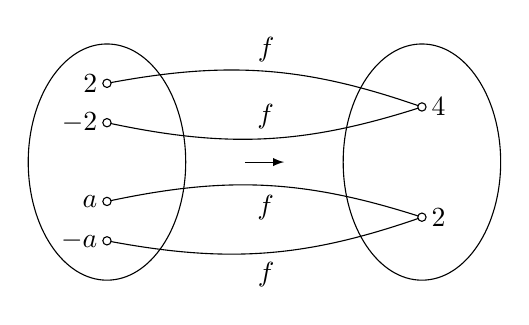
\begin{tikzpicture}[>=latex]
\draw (0,0) ellipse [x radius=1, y radius=1.5];
\draw (4,0) ellipse [x radius=1 ,y radius=1.5];

\draw(0,1)to [bend left=15] node[above]{$f$} (4,.7);
\draw (0,.5)to [bend left=-15]node[above]{$f$} (4,.7);
\draw (0,-1)to [bend left=-15]node[below]{$f$}(4,-.7);
\draw (0,-.5)to [bend left=15]node[below]{$f$} (4,-.7);

\draw[->](1.75,0)--(2.25,0);

\foreach \x/\xtext in {1/2,.5/-2,-.5/a,-1/-a}
{
    \draw (0,\x) [fill=white]circle (1.5pt)node[left]{$\xtext$};
}
\foreach \x/\xtext in {.7/4,-.7/2}
{
    \draw (4,\x) [fill=white]circle (1.5pt)node[right]{$\xtext$};
}
    \end{tikzpicture}
    \caption{}
\end{figure}


下面我们来说明具有怎样性质的函数才有反函数。

假如函数$y=f(x)$具有这样的性质:“若$x_1\ne x_2\; \Rightarrow\; f(x_1)\ne f(x_2)$, 也就是说对于定义域$X$中任意不同的$x_1$, $x_2$, 它们在值域$Y=f(X)$中的对应值$f(x_1)$, $f(x_2)$也不相同”。那么
对于$Y=f(X)$内任何一个$y$, 通过函数$f$, 可以逆对应出一
个且只有一个$x$, 使得$y$和这个$x$对应,这样一个函数叫做由
$X$到$Y=f(X)$的一一对应函数,或双射(满射且单射),简
称这个函数是\textbf{可逆}的。对于一个可逆函数$f:\; x\mapsto f(x)$, 我
们可以交换自变数与因变数的地位,于是对于$Y=f(X)$的
每一个$y$就有$X$内唯一一个逆象$x$, 这就是说我们得到了一
个新函数:
\[ g:\; Y=f(X)\mapsto X,\qquad \text{使得}\; y\mapsto x=g(y)\]
假如$y=f(x)$。

新函数和原来函数的这种关系可以用下图来说明:
\begin{center}
    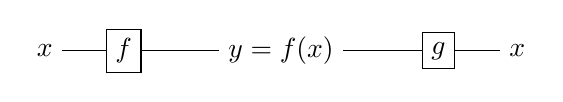
\begin{tikzpicture}
        \node (A) at (1,0) {$x$};
       \node[rectangle, draw] (B) at (2,0) {$f$};
       \node (C) at (4,0) {$y=f(x)$};
       \node[rectangle, draw] (D) at (6,0) {$g$};
       \node (E) at (7,0) {$x$};    
       \draw (A)--(B)--(C)--(D)--(E);
           \end{tikzpicture}
\end{center}


根据上面的分析,我们得到反函数的一般定义如下:
 
\begin{blk}{定义}
    设给了一个函数$y=f(x)$, 其定义域为$X$, 值域
为$Y=f(X)$, 如果对于$Y=f(X)$中每一个$y$值,都可以从关
系式$y=f(x)$确定唯一的一个$x$值,则得到一个定义在$Y=
f(X)$上而且把$f(X)=Y$映射到$X$上的以$y$为自变数的新函
数$x=g(y)$, 这个函数称为函数$y=f(x)$的反函数。
\end{blk}

不难理解$f$也是$g$的反函数,并且函数$y=f(x)$与它
的反函数$x=g(y)$组成的复合函数一定是一个恒等函数,即
\[ g\big(f(x)\big)=x,\qquad f\big(g(y)\big)= y\]
有时用符号$f^{-1}$表示反函数比较方便,如
\[f^{-1}\big(f(x)\big)=x,\qquad f\big(f^{-1}(y)\big)=y\]

按照函数$y=f(x)$的图象容易判断函数$y=f(x)$是否
有反函数存在,就是在值域$Y=f(X)$内,任意给一个值$y_0$,
作和$x$轴平行的直线$y=y_0$。如果函数$y=f(x),\; x\in X$的图
象和直线$y=y_0$的交点多于一个,那么这个函数的反函数就
不存在。如果只有一个交点,那么这个函数就有反函数。如
图8.22所示。

\begin{figure}[htp]
    \centering
    \begin{tikzpicture}[>=latex]
\begin{scope}
    \draw[->] (-2,0)--(4,0)node[right]{$x$};
        \draw[->] (0,-1)--(0,2)node[right]{$y$};
        \draw(-2,1)--(3,1)node[right]{$y=y_0$};
        \node at (-.25,-.25){$O$};
        \draw[ thick] plot[smooth] coordinates{(-1.7,-.5)(-1.0,.6)(0,1.2) (1.2,-.3)(1.6,-.5)(2,-.3) (2.5,1.2) };
    \node at (2.5,1.2)[above]{$y=f(x)$是不可逆的};
\end{scope}
\begin{scope}[yshift=-3.5cm]
    \draw[->] (-2,0)--(4,0)node[right]{$x$};
    \draw[->] (0,-1)--(0,2)node[right]{$y$};
    \draw(-2,1)--(3,1)node[right]{$y=y_0$};
    \node at (-.25,-.25){$O$};
    \draw[ thick] plot[smooth] coordinates{(-1.5,-.5)(-.7,.3) (0,.5) (1.3,.7) (2.5,1.8)};
    \node at (2.5,1.8)[above]{$y=f(x)$是可逆的};
\end{scope}        
    \end{tikzpicture}
    \caption{}
\end{figure}

现在我们来研究互为反函数的图象的关系,因为互为反
函数的两个函数$y=f(x)$和$x=g(y)$事实上就是同一个关系,在
几何上就是同一条曲线。例如函数$y=2x+3$的图象和它的反
函数$x=\frac{1}{2}(y-3)$的图象就是通过两个
点$\left(-\frac{3}{2},0\right)$, $(0,3)$的同一条直线$2x-y+3=0$, 只是就函数$y=f(x)=2x+
3$的图象去看,横轴是自变量轴,而就反函数$x=g(y)=\frac{1}{2}
(y-3)$的图象来看,纵轴是自变量轴,但是在同一个坐标系
内,一般我们总规定用横坐标$x$表示自变数,纵坐标$y$表示
因变数,所以我们还需要把反函数关系式$x=g(y)$的$x,y$对
调一下,得到习惯上的反函数$y=g(x)$。我们也称$y=g(x)$
是$y=f(x)$的反函数,当然反过来$y=f(x)$也是$y=g(x)$的反
函数,例如函数$y=2x+3$和 $y=\frac{1}{2}(x-3)$互为反函数。

函数$y=f(x)$和它的反函数$y=f^{-1}(x)$的图象之间有如
下关系:

若点$(a,b)$在曲线$y=f(x)$上,那么点$(b,a)$就在曲线
$y=f^{-1}(x)$上。

事实上,因为点$(a,b)$在曲线$y=f(x)$上,所以$b=f(a)$
成立,此等式也可以写成$a=f^{-1}(b)$, 这表示点$(b,a)$在曲
线$y=f^{-1}(x)$上,于是当点$(a,b)$走遍曲线$y=f(x)$时,点
$(b,a)$就走遍曲线$y=f^{-1}(x)$. 通过初等几何的方法可以证
明点$(a,b)$和$(b,a)$关于第一象限角和第三象限角的平分线
$y=x$对称。因此,为了得到反函数$y=f^{-1}(x)$的图象,我
们只要把$y=f(x)$的图象关于直线$y=x$反射过来就可以。如
图8.23所示。
\begin{figure}[htp]
    \centering
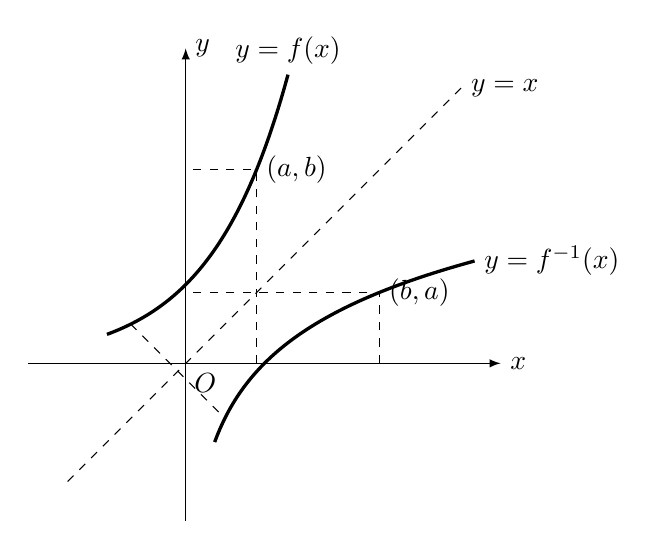
\begin{tikzpicture}[>=latex]
    \draw[->] (-2,0)--(4,0)node[right]{$x$};
    \draw[->] (0,-2)--(0,4)node[right]{$y$};
    \draw [domain=-1:1.3, samples=100,  very thick]plot(\x, {exp(\x)});
    \draw [domain=exp(-1):exp(1.3), samples=100,  very thick]plot(\x, {ln(\x)});
\draw[dashed] (-1.5,-1.5)--(3.5,3.5)node[right]{$y=x$};
\draw[dashed] (2.46,0)--(2.46,.9)node[right]{$(b,a)$}--(0,.9);
\draw[dashed] (.9,0)--(.9,2.46)node[right]{$(a,b)$}--(0,2.46);
\draw[dashed]  (-.7,.5)--(.5,-.7);
\node at (.25,-.25){$O$};
\node at (3.67,1.3)[right]{$y=f^{-1}(x)$};
\node at (1.3,3.67)[above]{$y=f(x)$};
\end{tikzpicture}
    \caption{}
\end{figure}


最后,我们给出一个反函数定理:

\begin{blk}{定理}
    设$y=f(x)$在闭区间$[a,b]$上严格递增(递减)
且连续,又$f(a)=\alpha$, $f(b)=\beta$, 则在闭区间$[\alpha,\beta]$  上存在着
$y=f(x)$的反函数$x=f^{-1}(y)$, 又$x=f^{-1}(y)$在$[\alpha,\beta]$  (或$[\beta,\alpha]$)上也是严格递增(或递减)且连续的。
\end{blk}

\begin{proof}
\begin{enumerate}
\item 先证$y=f(x)$的值域是闭区间$[\alpha,\beta]$, 设$y$
是$[\alpha,\beta]$中任意一点,如果$y=\alpha$或$\beta$,那么相应的$x=a$或$b$, 即
有$f(a)=\alpha$或$f(b)=\beta$, 换言之,$\alpha ,\beta$  在$f(x)$的值域中。又如
果$\alpha=f(a)<y_0<f(b)=\beta  $, 由连续函数中间值定理,在$[a,
b]$之间必存在一点$x_0$满足$f(x_0)=y_0$, 即$[\alpha ,\beta]$  内任一点都
属于值域$f([a,b])$, 又如果$y_0\notin [\alpha ,\beta]$, 那么由严格递增
性得出,它不可能是任一点$x\in [a,b]$的象,这就证明了
$f(x)$的值域是$[\alpha,\beta]$, 因此,连续递增函数$f:[a,b]\mapsto [\alpha ,\beta]$是满射的。

\item 再证$f$是单射的,因为一个严格递增函数$f$满足
条件:$$x_1<x_2\quad \Rightarrow\quad f(x_1)<f(x_2)$$ 即自变数的值与函数值是一对
一的,所以$f$是单射的。

由上可知函数$f$是可逆的,因此存在一个反
函数$f^{-1}:[\alpha,\beta]\mapsto [a,b]$, 其中$x=f^{-1}(y)$.
\item 证明$f^{-1}$的递增性。

假设$y_1,y_2$是$[\alpha,\beta]$内的两个数,并且$y_1<y_2$, 又设$x=f^{-1}(y_1)$, $x_2=f^{-1}(y_2)$, 对于这两数$x_1$和$x_2$只有三种可能:
$x_1<x_2$, $x_1=x_2$, $x_1>x_2$。

如果$x_1\ge x_2$, 由于$f$的递增性质,知道
\[y_1=f(x_1)\ge f(x_2)=y_2\]
这与$y_1<y_2$的假设矛盾,因此,$x_1<x_2$, 即
\[y_1<y_2 \quad \Rightarrow\quad f^{-1}(y_1)=x_1<x_2=f^{-1}(y_2)\]
这就证明了$x=f^{-1}(y)$是$[\alpha,\beta]$上的递增函数。
\item 最后还应证明$x=f^{-1}(y)$在$[\alpha,\beta]$上连续,但是
在高中阶段,我们不深究,同学只要知道结论就可以了。
\end{enumerate}    
\end{proof} 


一般来说,一个函数可以分成分段单调的几支,对于每
一支得一反函数。

例如,函数$y=f(x)=x^2,\; x\in\mathbb{R}$在区间$[0,+\infty)$或
$(-\infty,0]$上连续和严格单调。因为$[0,b]\subset [0,+\infty)$和
$[-b,0]\subset (-\infty,0]$,这个$b$是任意大的正数,因此$y=x^2,\; x\in\mathbb{R}$的两个分段$y=f_1(x)=x^2,\; x\in [0,b]$和$y=f_2(x)=x^2,\; x\in[-b,0)$根据反函数存在定理,分别有反函数:
\[\begin{split}
    x&=f^{-1}_1(y)=\sqrt{y},\qquad y\in [0,b^2]\\    
    x&=f^{-1}_2(y)=-\sqrt{y},\qquad y\in [0,b^2]\\
\end{split}\]
但是当$b\to+\infty$时,$b^2\to+\infty$, 所以,
\begin{itemize}
    \item 连续和递增的一段$y=f_1(x)=x^2,\; x\in[0,+\infty)$的反函
数是$x=f_1^{-1}(y)=\sqrt{y},\; y\in [0,+\infty)$, 它是连续的和严格
递增的;
\item 连续和递减的一段$y=f_2(x)=x^2,\; x\in(-\infty,0]$的反函数
是$x=f_2^{-1}(y)=-\sqrt{y},\; y\in[0,+\infty)$, 它是连续的和严格
递减的。
\end{itemize}

将$f_1^{-1}$和$f_2^{-1}$中的$x$和$y$对调后,便得到$f_1$和$f_2$的矫形的
反函数,(见图8.24)。
\[\begin{split}
    y&=f^{-1}_1(x)=\sqrt{x},\qquad y\in [0,+\infty)\\    
    y&=f^{-1}_2(x)=-\sqrt{x},\qquad y\in [0,+\infty)\\
\end{split}\]

\begin{figure}[htp]
    \centering
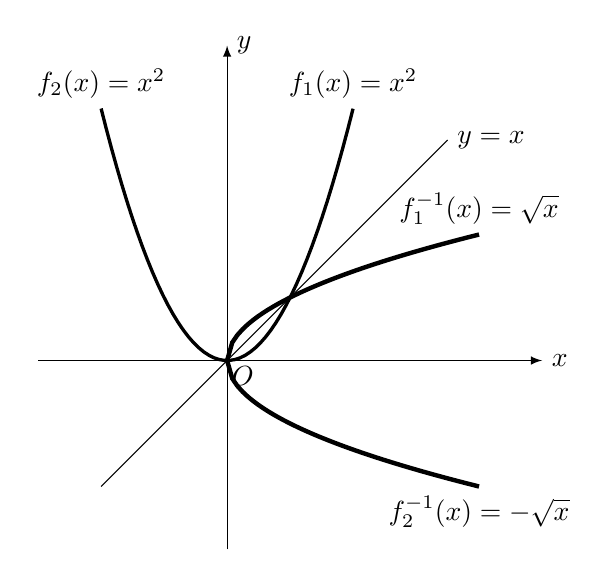
\begin{tikzpicture}[>=latex, scale=.8]
    \draw[->] (-3,0)--(5,0)node[right]{$x$};
    \draw[->] (0,-3)--(0,5)node[right]{$y$};
\node at (.25,-.25){$O$};
\draw [domain=-2:2, samples=50, very thick]plot(\x, {\x*\x});
\draw [domain=0:4, samples=50,ultra thick]plot(\x, {sqrt(\x)});
\draw [domain=0:4, samples=50,ultra thick]plot(\x, {-sqrt(\x)});
\draw (-2,-2)--(3.5,3.5)node[right]{$y=x$};
\node at (-2,4)[above]{$f_2(x)=x^2$};
\node at (2,4)[above]{$f_1(x)=x^2$};
\node at (4,-2)[below]{$f_2^{-1}(x)=-\sqrt{x}$};
\node at (4,2)[above]{$f_1^{-1}(x)=\sqrt{x}$};

\end{tikzpicture}    
    \caption{}
\end{figure}


一般地,函数$y=f(x)=x^n,\; (n\in\mathbb{N})$在半开区间$[0,+\infty)$上
连续和严格递增,函数$f$有反函数
\[x=f^{-1}(y)=\sqrt[n]{y}=y^{\tfrac{1}{n}},\qquad y\in [0,+\infty)\]
它是连续的和严格递增的。

在图8.25中,我们画出几个幂函数和它们的反函数的
图象:
\begin{figure}[htp]
    \centering
\begin{tikzpicture}[>=latex, scale=2]
    \draw[->] (0,0)--(3.5,0)node[right]{$x$};
    \draw[->] (0,0)--(0,3.5)node[right]{$y$};
\draw [domain=0:1.8, samples=100, thick] plot (\x, {\x^2});
\draw [domain=0:1.5, samples=100, very thick] plot (\x, {\x^3});
\draw [domain=0:1.35, samples=100, ultra thick] plot (\x, {\x^4});
\draw [domain=0:3, samples=100, semithick] plot (\x, {\x});
\draw [domain=0:3.25, samples=100, thick] plot (\x, {\x^(1/2)});
\draw [domain=0:3.25, samples=100, very thick] plot (\x, {\x^(1/3)});
\draw [domain=0:3.25, samples=100, ultra thick] plot (\x, {\x^(1/4)});
\foreach \x in {1,2,3}
{
    \draw (\x,0)node[below]{$\x$}--(\x,.05);
    \draw(0,\x)node[left]{$\x$}--(.05,\x);
}
\node at (-.1,-.1){$O$};
\node at (3,3)[right]{$y=x$};
\node at (1.2,.9){$(1,1)$};
\node at (1.8,{1.8^2})[right]{$y=x^2$};
\node at (1.5,{1.5^3})[above]{$y=x^3$};
\node at (1.35,{1.35^4})[left]{$y=x^4$};
\node at (3.25,{3.25^(1/2)})[above]{$y=x^{\tfrac{1}{2}}$};
\node at (3.25,{3.25^(1/3)})[right]{$y=x^{\tfrac{1}{3}}$};
\node at (3.25,{3.25^(1/4)})[below]{$y=x^{\tfrac{1}{4}}$};




\end{tikzpicture}    
    \caption{}
\end{figure}






\section*{习题8.4}
\addcontentsline{toc}{subsection}{习题8.4}
\begin{enumerate}
\item 下列函数在哪些范围内是严格单调的?
\begin{multicols}{2}
  \begin{enumerate}
    \item $f(x)=x^3$
    \item $\varphi(x)=x^4$
    \item $y=\sqrt{x}$
    \item $y=\sqrt[3]{x}$
    \item $f(x)=|x+1|$
\end{enumerate}  
\end{multicols}


\item 对于下列各函数分别找出它们的最大定义域和值域
使得它们有反函数,并分别写出它们的变数$x$表出的反
函数。
\begin{multicols}{2}
    \begin{enumerate}
      \item $y=\sqrt{2x+1}$
      \item $y=x^{\tfrac{3}{2}}$
      \item $y=x^2-1$
      \item $y=\sqrt{1-x^2}$
      \item $f(x)=\frac{x}{1-x^2},\quad -1<x<1$
  \end{enumerate}  
  \end{multicols}

\item 作出下列各函数和它的反函数的图象:
\begin{multicols}{2}
    \begin{enumerate}
      \item $y=x^{\tfrac{1}{2}}\quad (x\ge 0)$
      \item $y=\frac{x+1}{x}\quad (x\ne 0)$
      \item $y=\frac{x}{x+1}\quad (x\ne -1)$
  \end{enumerate}  
  \end{multicols}

\item 证明,当且仅当$ad-bc\ne 0$时,$f(x)=\frac{ax+b}{cx+d},\; \left(x\ne -\frac{d}{c}\right)$
是单射的,并求它的反函数。又在什么条件下,
$f(x)$的反函数等于原来函数。
\item \begin{enumerate}
\item 求$f(x)=\frac{2x-5}{x-3}$
的反函数$f^{-1}(x)$。
\item 已知函数$f(x)=\frac{2x-5}{x-3}$
的值域是$\{f(x)|f(x)\le 0,\; f(x)\ge 4\}$, 求$f(x)$的定义域。
\item 设函数$g(x)=\frac{ax-4}{x+b}$的反函数是$g^{-1}(x)=\frac{3x+c}{-x+2}$,求实数$a,b,c$的值。
\end{enumerate}

\item $f(x)=\begin{cases}
    -x,& x\ge 0\\ x^2& x<0
\end{cases}$
给出由实数集$\mathbb{R}$到$\mathbb{R}$的一个函
数$f$。
\begin{enumerate}
    \item 设$q(x)$是$f$和$f$的复合函数,用$x$的式子表示$q(x)$.
    \item 设$q(x)$的反函数是$q^{-1}(x)$, 用$x$的式子表示$q^{-1}(x)$.
\end{enumerate}
\end{enumerate}






